\documentclass[
  shortnames]{jss}

%% recommended packages
\usepackage{orcidlink,thumbpdf,lmodern}

\usepackage[utf8]{inputenc}

\author{
Rebecca Fisher~\orcidlink{0000-0001-5148-6731}\\Australian Institute of Marine Science \And Diego R. Barneche~\orcidlink{0000-0002-4568-2362}\\Australian Institute of Marine Science \And Gerard Ricardo~\orcidlink{0000-0002-7761-0806}\\University of Queensland \And David Fox~\orcidlink{0000-0002-3178-7243}\\University of Melbourne
}
\title{\pkg{bayesnec}: An \proglang{R} Package for CR Modelling and Estimation of toxicity metrics}

\Plainauthor{Rebecca Fisher, Diego R. Barneche, Gerard Ricardo, David Fox}
\Plaintitle{bayesnec: An R Package for CR Modelling and Estimation of No-Effect-Concentrations}
\Shorttitle{\pkg{bayesnec}: An R Package for CR Modelling}


\Abstract{
The \pkg{bayesnec} package has been developed for \proglang{R} to fit concentration(dose) - response curves (CR) to toxicity data for the purpose of deriving no-effect-concentration (NEC), no-significant-effect-concentration (NSEC), and effect-concentration (of specified percentage `x', ECx) thresholds from non-linear models fitted using Bayesian Hamiltonian Monte Carlo (HMC) via \pkg{brms} \citep{Burkner2017, Burkner2018} and \pkg{rstan} \citep{rstan2021} or \pkg{cmdstanr} \citep{cmdstanr2022}. In \pkg{bayesnec} it is possible to fit a single model, custom models-set, specific model-set or all of the available models. When multiple models are specified the \code{bnec} function returns a model weighted average estimate of predicted posterior values. A range of support functions and methods is also included to work with the returned single, or multi-model objects that allow extraction of raw, or model averaged predicted, NEC, NSEC and ECx values and to interrogate the fitted model or model-set. By combing Bayesian methods with model averaging, \pkg{bayesnec} provides a single estimate of toxicity and assocaited uncertainty that can be directly integrated into risk assessment frameworks.
}

\Keywords{concentration-response, toxicity, no-effect-concentration, \proglang{R}, Bayesian, non-linear modelling}
\Plainkeywords{concentration-response, toxicity, no-effect-concentration, R, Bayesian, non-linear modelling}

%% publication information
%% \Volume{50}
%% \Issue{9}
%% \Month{June}
%% \Year{2012}
%% \Submitdate{}
%% \Acceptdate{2012-06-04}

\Address{
    Rebecca Fisher\\
    University of Western Australia\\
    Australian Institute of Marine Science,Crawley, WA, Australia\\
  E-mail: \email{r.fisher@aims.gov.au}\\
  
      Diego R. Barneche\\
    University of Western Australia\\
    Australian Institute of Marine Science,Crawley, WA, Australia\\
  
  
      Gerard Ricardo\\
    Australian Institute of Marine Science\\
    The University of Queensland,St Lucia, Qld, Australia\\
  
  
      David Fox\\
    Environmetrics Australia\\
    University of Melbourne,Parkville, Victoria, Australia\\
  
  
  }


% tightlist command for lists without linebreak
\providecommand{\tightlist}{%
  \setlength{\itemsep}{0pt}\setlength{\parskip}{0pt}}

% From pandoc table feature
\usepackage{longtable,booktabs,array}
\usepackage{calc} % for calculating minipage widths
% Correct order of tables after \paragraph or \subparagraph
\usepackage{etoolbox}
\makeatletter
\patchcmd\longtable{\par}{\if@noskipsec\mbox{}\fi\par}{}{}
\makeatother
% Allow footnotes in longtable head/foot
\IfFileExists{footnotehyper.sty}{\usepackage{footnotehyper}}{\usepackage{footnote}}
\makesavenoteenv{longtable}



\usepackage{amsmath}
\usepackage{float}
\usepackage{caption}

\begin{document}



\hypertarget{introduction}{%
\section{Introduction}\label{introduction}}

Concentration-response (CR) modelling (also known as dose-response modelling or dose-response analysis) is a key tool for assessing toxicity and deriving the toxicity thresholds used in the risk assessments that underpin protection of human health and the environment. It is widely used in the disciplines of pharmacology, toxicology and ecotoxicology, where parametric non-linear regression methods are used to model response data of interest, with the resulting fitted models used to estimate critical thresholds of concern. These thresholds may be used directly to assess risk \citep[e.g see][]{fisher2018c}, or are subsequently incorporated into a broader population-level risk assessment framework \citep[e.g.][]{Warne2015}. Typical thresholds derived from CR modelling include the effect-concentration of defined percentage `x' (ECx) and the no-effect-concentration (NEC), the latter being the generally preferred option \citep{Fox2008, Warne2015, Warne2018c}. In addition, the no-significant-effect-concentration (NSEC) has also been recently defined \citep{Fisher2023}, and may represent a good alternative estimate of ``no-effect'' concentrations when the threshold models required to derive true NEC estimates are not appropriate \citep{Fisher2023, fisher2023ieam}.

In qualitative terms, CR models are typically a decreasing function of concentration, whereby the response may remain relatively stable for the initial portion of the curve, and then decays at some rate to zero (or some other lower bound at high concentration). An example is death of an organism resulting from ever increasing concentrations of a toxic pollutant. However, often the underlying mechanisms describing CR relationships are not known, and therefore numerous alternative non-linear CR equations have been proposed (e.g.~models in \pkg{drc}, \citet{Ritz2016}). These can be broadly grouped into two main ``model categories'' (see below Section \ref{mdbnc}) for the mathematical definition of each model): NEC models---threshold models which contain a step function comprising the ``break-point'' after which the predictor systematically alters the response \citep{Fox2010}; and Smooth transition models that are typically used for estimating effect concentrations of a specified effect (e.g.~ECx- models). They may or may not encompass the EC\textsubscript{50} as a parameter \citep{Ritz2016}. Each of these two groups can be further split into two categories depending on whether the initial portion of the curve is flat, or increasing---the latter being known as hormesis models \citep{Ritz2016}.

The above model categories mostly comprise non-linear equations, thereby increasing the technical complexity of model fitting. CR experimental designs are often also complex, and may require the addition of multi-level, hierarchical effects. Examples might include a random offset to model non-independence of replicates housed together in tanks, or where there are repeated measurements on individual genotypes of a test species. Additionally, CR data are of varied nature, with the measured response data taking a wide range of natural distributions. For instance, response data may be unbounded continuous (e.g., growth when shrinkage is possible), or positive continuous (e.g., growth in the absence of shrinkage), proportional (e.g., fertilization success), or binary (e.g., survival). To the best of our knowledge, there is no open-source statistical software dedicated to CR modelling which allows for appropriate model and error distribution specification depending on the input data. However, there is a wide array of multi-purpose packages for fitting non-linear generalised hierarchical models in \proglang{R}. For example (to list a few), \pkg{nlme} \citep{pinheiro2021}, \pkg{lme4} \citep{pinheiro2021}, \pkg{rjags} \citep{Su2015} and \pkg{rstan} \citep{rstan2021}.

While CR modelling can be carried out using generic non-linear modelling software packages, this can be cumbersome in practice, requiring extensive manual programming to obtain the necessary, often relatively standard outputs. The \pkg{drc} package \citep{Ritz2016} was developed as a user friendly frequentist based solution to CR modelling in \proglang{R}, and is currently widely used across a range of disciplines. \pkg{drc} implements a broad range of non-linear CR models, provides facilities for ranking model fits based on AIC \citep{Burnham2002}, joint modelling of multiple response curves, and supports a range of estimation procedures \citep{Ritz2016}. Section \ref{bnchmrk} provides a formal comparison between \pkg{drc} and \pkg{bayesnec} standard output using default argument values.

Estimates of uncertainty in parameters and derived thresholds are critical for effective integration of threshold estimates into risk assessment and formal decision frameworks \citep{fisher2018c}. Bayesian methods allow robust quantification of uncertainty with intuitive and direct probabilistic meaning \citep{Ellison1996}, and are therefore an excellent platform for CR modelling in most settings. Furthermore, the posterior draws generated through Bayesian model fitting methods provide a rich resource that can be used to explore synergistic and antagonistic impacts \citep{Fisher2019d, flores2021}, propagate toxicity estimate uncertainty \citep{Charles2020a, Gottschalk2013}, and test hypotheses of no-effect \citep{Thomas2006}.

There is a wide array of packages available for Bayesian model fitting via Markov chain Monte Carlo methods, including \proglang{WinBUGS} \citep{Lunn2000}, \proglang{JAGS} \citep{Plummer2003} and \proglang{Stan} \citep{Carpenter2017}, that seamlessly interface with R through packages such as \pkg{R2WinBUGS}, \pkg{R2jags} \citep{Su2015} and \pkg{rstan} \citep{rstan2021}. These packages require coding in \proglang{R} and additional model specification in custom languages---which might involve non trivial coding, extensive debugging and optimisation that is often time consuming and requires specialist expertise. All of which might add a learning/application barrier to many potential users. Several extension packages which aim to reduce that barrier have recently become available, principally \pkg{brms} \citep{Burkner2017}, that allows a broad range of models to be easily fitted using \pkg{rstan} \citep{rstan2021} or \pkg{cmdstanr} \citep{cmdstanr2022} through simpler \pkg{lme4}-like formula syntax. However, even with packages like \pkg{brms}, Bayesian model fitting can be difficult to automate across all potential usage cases, particularly with respect to specifying valid initial parameter values and appropriate priors. In addition, as was the motivation for the development of the \pkg{drc} package in the frequentist setting, the \proglang{R} code required for fitting non-linear models and extracting the relevant outputs (e.g.~NEC, ECx) and their standard errors can be cumbersome in practice, and even more so in the Bayesian setting where model fits contain multiple posterior draws.

The greater complexity associated with Bayesian model fitting has likely hindered the uptake of Bayesian statistics for CR threshold derivation across the broader ecotoxicology and toxicology communities, who may not have access to specialist statistical expertise \citep{Fisher2019}. \pkg{bayesnec} version 2.1.0.3 (available on CRAN) builds upon an implementation of the NEC model described in \citet{Fox2010} and \citet{Pires2002}. The \pkg{bayesnec} package provides an accessible interface specifically for fitting NEC and ECx and other CR models using Bayesian methods. A variety of models can be specified based on the known distribution of the ``concentration'' or ``dose'' variable (the predictor, x) as well as the ``response'' (y) variable. The model formula, including priors and initial values required to call \pkg{brms} are automatically generated based on information contained in the supplied data. A range of tools is supplied to aid the user in interrogating model fits, plotting and generating predicted values, as well as extracting the standard outputs, such as NEC and ECx - either as a full posterior draw or in summary form.

\hypertarget{technical-details}{%
\section{Technical details}\label{technical-details}}

In Bayesian inference, model parameters and their inherent uncertainty are estimated as statistical probability distributions. This is achieved by combining an a-priori probability distribution for each parameter (the `priors', \(p(\theta)\)) with the likelihood of the observed data, \(D\), given the model parameters, \(p(D | \theta)\), to yield a so-called posterior probability distribution, \(p(\theta | D)\)

\begin{equation}
  p(\theta | D) = \frac{p(D | \theta) p(\theta)}{\int_{\theta} p(D | \theta) p(\theta) d \theta} \propto p(D | \theta) p(\theta).
  \label{eqn1}
\end{equation}

In many cases, the denominator (a.k.a. ``evidence'' or ``marginal'') is analytically intractable, and therefore we resort to numerical approximations such as Markov Chain Monte Carlo (MCMC). \pkg{bayesnec} uses the extensive functionality of the \pkg{brms} package to write model code as well as fit models via a \proglang{Stan} program \citep{stan2021}, which typically defines a Bayesian posterior as a log density function conditioned on the data. \proglang{Stan} employs Hamiltonian Monte Carlo (HMC)---a type of MCMC algorithm---for its fitting mechanism, and automatically optimizes the discretization time parameter to match an acceptance-rate target using the no-U-turn sampling (NUTS) algorithm \citep{hoffman2014}. \pkg{bayesnec} first takes the input model or model-set (via its custom formula class, \code{bayesnecformula}) in conjunction with potential user-defined hierarchical effects, to generate an object of class \code{brmsformula}. Then, based on the package-(or user-)specified priors, and response model distribution, it calls \pkg{brms} \citep{Burkner2017, Burkner2018} to generate the \proglang{Stan} program code and fit the model through either \pkg{rstan} \citep{rstan2021} or \pkg{cmdstanr}\citep{cmdstanr2022}. In doing so, \pkg{bayesnec} (as of version 2.1.0.3) allows for response variables to be modelled with a variety of statistical distributions: Gaussian, Poisson, Binomial, Gamma, Negative-binomial, Beta and Beta-binomial. Future implementations of \pkg{bayesnec} might include additional distributions which are currently only implemented in \pkg{brms}. In addition to greater flexibility in the available response distributions, \pkg{bayesnec} includes a larger set of 23 NEC- and ECx- models (see below), including many of the commonly-used models in \pkg{drc} \citep{Ritz2016}.

\subsection[Models in bayesnec]{Models in \pkg{bayesnec}}\label{mdbnc}

Where possible we have aimed for consistency in the interpretable meaning of the individual parameters across models. Across the currently implemented model sets, models contain from two (basic linear or exponential decay, see \code{ecxlin} or \code{ecxexp}) to five possible parameters (\code{nechorme4}), including:

\(\tau = \text{top}\), usually interpretable as either the response's intercept or the upper plateau representing the mean concentration of the response at zero concentration;

\(\eta = \text{NEC}\), the No-Effect-Concentration value (the concentration value where the breakpoint in the regression is);

\(\beta = \text{beta}\), generally the exponential decay rate of response, either from 0 concentration or from the estimated \(\eta\) value, with the exception of the \code{neclinhorme} model where it represents a linear decay from \(\eta\) because slope (\(\alpha\)) is required for the linear increase (see below);

\(\delta = \text{bottom}\), representing the lower asymptotic response at infinite concentration;

\(\alpha = \text{slope}\), the linear decay rate in the models \code{neclin} and \code{ecxlin}, or the linear increase rate prior to \(\eta\) for all hormesis models;

\(\omega\) = \(\text{EC\textsubscript{50}}\), notionally the 50\% effect concentration but may be influenced by scaling and should therefore not be strictly interpreted as such,

\(\epsilon = \text{d}\), the exponent in the \code{ecxsigm} and \code{necisgm} models, and

\(\phi = \text{f}\) A scaling exponent exclusive to model \code{ecxll5}.

In addition to the model parameters, all \emph{NEC}- models have a step (indicator) function used to define the breakpoint in the regression, which can be defined as

\[
f(x_i, \eta) = \begin{cases} 
      0, & x_i - \eta < 0 \\
      1, & x_i - \eta \geq 0 \\
   \end{cases}
\]

Note that strictly positive parameters (for example, \(\beta\) and \(\epsilon\)) have been transformed as exponential functions to allow the use of normal priors and stabilize model fitting.

\subsubsection[ECx models]{ECx models}\label{ecx-models}

\code{ecxlin} is a basic linear decay model, given by the equation:
\(y_i = \tau - e^{\alpha} x_i\)
with the following \code{brmsformula}: \code{y ~ top - exp(slope) * x}. Because the model contains linear predictors it is not suitable for 0--1 bounded data (i.e., Binomial and Beta families with an \code{"identity"} link function). As the model includes a linear decline with concentration, it is also not suitable for 0 bounded data (Gamma, Poisson, Negative Binomial with an \code{"identity"} link).

\code{ecxexp} is a basic exponential decay model, given by the equation: \(y_i = \tau e^{-e^{\beta} x_i}\)
with the following \code{brmsformula}: y \textasciitilde{} top * exp(-exp(beta) * x). The model is 0-bounded, thus not suitable for Gaussian response data or the use of a \code{"logit"} or \code{"log"} link function.

\code{ecxsigm} is a simple sigmoidal decay model, given by the equation:
\(y_i = \tau e^{-e^{\beta} x_i^{e^\epsilon}}\)
with the following \code{brmsformula}: y \textasciitilde{} top * exp(-exp(beta) * x\^{}exp(d)). The model is 0-bounded, thus not suitable for Gaussian response data or the use of a \code{"logit"} or \code{"log"} link function.

\code{ecx4param} is a 4-parameter sigmoidal decay model, given by the equation:
\(y_i = \tau + (\delta - \tau)/(1 + e^{e^{\beta} (\omega - x_i)})\)
with the following \code{brmsformula}: y \textasciitilde{} top + (bot - top)/(1 + exp((ec50 - x) * exp(beta)))

\code{ecxwb1} is a 4-parameter sigmoidal decay model which is a slight reformulation of the Weibull1 model of \citet{Ritz2016}, given by the equation:
\(y_i = \delta + (\tau - \delta) e^{-e^{e^{\beta} (x_i - \omega)}}\)
with the following \code{brmsformula}: y \textasciitilde{} bot + (top - bot) * exp(-exp(exp(beta) * (x - ec50)))

\code{ecxwb1p3} is a 3-parameter sigmoidal decay model, equivalent to the \code{ecxwb1} model where \(\delta\) (bottom) is defined as 0, given by the equation:
\(y_i = {0} + (\tau - {0}) e^{-e^{e^{\beta} (x_i - \omega)}}\)
with the following \code{brmsformula}: y \textasciitilde{} 0 + (top - 0) * exp(-exp(exp(beta) * (x - ec50))). The model is 0-bounded, thus not suitable for Gaussian response data or the use of a \code{"logit"} or \code{"log"} link function.

\code{ecxwb2} is a 4-parameter sigmoidal decay model which is a slight reformulation of the Weibull2 model of \citet{Ritz2016}, given by the equation:
\(y_i = \delta + (\tau - \delta) (1 - e^{-e^{e^{\beta} (x_i - \omega)}})\)
with the following \code{brmsformula}: y \textasciitilde{} bot + (top - bot) * (1 - exp(-exp(-exp(beta) * (x - ec50)))). While very similar to the \code{ecxwb1} \citep[according to][]{Ritz2016}, fitted \code{ecxwb1} and \code{ecxwb2} models can differ slightly.

\code{ecxwb2p3} is a 3-parameter sigmoidal decay model, equivalent to the \code{ecxwb2} model where the parameter \(\delta\) (bot) is defined as 0, given by the equation:
\(y_i = {0} + (\tau -{0}) (1 - e^{-e^{e^{\beta} (x_i - \omega)}})\)
with the following \code{brmsformula}: y \textasciitilde{} 0 + (top - 0) * (1 - exp(-exp(-exp(beta) * (x - ec50)))). The model is 0-bounded, thus not suitable for Gaussian response data or the use of a logit or log link function.

\code{ecxll5} is a 5-parameter sigmoidal log-logistic decay model, which is a slight reformulation of the LL.5 model of \citet{Ritz2016}, given by the equation:
\(y_i = \delta + (\tau - \delta) / (1 + e^{-e^{\beta} (x_i - \omega)})^{e^\phi}\)
with the following \code{brmsformula}: y \textasciitilde{} bot + (top - bot)/(1 + exp(exp(beta) * (x - ec50)))\^{}exp(f).

\code{ecxll4} is a 4-parameter sigmoidal log-logistic decay model, equivalent to the the \code{ecxll5} model, but where the parameter \(\phi\) (f) is defined as 0, given by the equation:
\(y_i = \delta + (\tau - \delta)/ (1 + e^{e^{\beta} (x_i - \omega)})\)
with the following \code{brmsformula}: y \textasciitilde{} bot + (top - bot)/(1 + exp(exp(beta) * (x - ec50))).

\code{ecxll3} is a 3-parameter sigmoidal log-logistic decay model, equivalent to the the \code{ecxll5} model, but where the parameters \(\phi\) (f) and \(\delta\) (bot) are both defined as 0, given by the equation:
\(y_i = 0 + (\tau - 0)/ (1 + e^{e^{\beta} (x_i - \omega)})\)
with the following \code{brmsformula}: y \textasciitilde{} 0 + (top - 0)/(1 + exp(exp(beta) * (x - ec50))).
The model is 0-bounded, thus not suitable for Gaussian response data or the use of a \code{"logit"} or \code{"log"} link function.

\code{ecxhormebc5} is a 5 parameter log-logistic model modified to accommodate a non-linear hormesis at low concentrations. It has been modified from to the ``Brain-Cousens'' (BC.5) model of \citet{Ritz2016}, given by the equation:
\(y_i = \delta + (\tau - \delta + e^{\alpha} x)/ (1 + e^{e^{\beta} (x_i - \omega)})\)
with the following \code{brmsformula}: y \textasciitilde{} bot + (top - bot + exp(slope) * x)/(1 + exp(exp(beta) * (x - ec50))).

\code{ecxhormebc4} is a 5-parameter log-logistic model similar to the \code{exchormebc5} model but with a lower bound \(\delta\) (bot) of 0, given by the equation:
\(y_i = 0 + (\tau - 0 + e^{\alpha} x)/ (1 + e^{e^{\beta} (x_i - \omega)})\)
with the following \code{brmsformula}: y \textasciitilde{} 0 + (top - 0 + exp(slope) * x)/(1 + exp(exp(beta) * (x - ec50))). The model is 0-bounded, thus not suitable for Gaussian response data or the use of a \code{"logit"} or \code{"log"} link function.

\begin{figure}[ht]
  \centering
  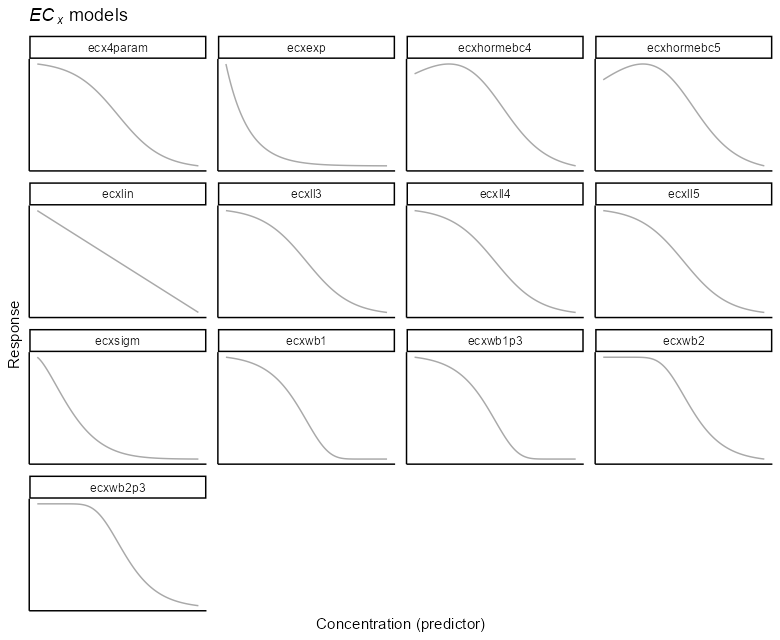
\includegraphics[width=1\textwidth]{../vignettes/vignette-fig-exmp2b-theoretical_ecx_curves.png}
  \caption{Representative shapes of currently implemented \pkg{bayesnec} \textit{EC\textsubscript{x}} models.}
  \label{fig1}
\end{figure}

\subsubsection[NEC models]{NEC models}\label{nec-models}

\code{neclin} is a basic linear decay model equivalent to \code{ecxlin} with the addition of the NEC step function, given by the equation:
\(y_i = \tau - e^{\alpha} \left(x_i - \eta \right) f(x_i, \eta)\)
with the following \code{brmsformula}: y \textasciitilde{} top - exp(slope) * (x - nec) * step(x - nec). Because the model contains linear predictors it is not suitable for 0--1 bounded data (Binomial and Beta distributions with \code{"identity"} link). As the model includes a linear decline with concentration, it is also not suitable for 0--\(\infty\) bounded data (Gamma, Poisson, Negative Binomial with \code{"identity"} link).

\code{nec3param} is a basic exponential decay model equivalent to \code{ecxexp} with the addition of the NEC step function, given by the equation:
\(y_i = \tau e^{-e^{\beta} \left(x_i - \eta \right) f(x_i, \eta)}\)
with the following \code{brmsformula}: y \textasciitilde{} top * exp(-exp(beta) * (x - nec) * step(x - nec)). For Binomial-distributed response data in the case of \code{"identity"} link this model is equivalent to that in \citet{Fox2010}. The model is 0-bounded, thus not suitable for Gaussian response data or the use of a \code{"logit"} or \code{"log"} link function.

\code{nec4param} is a equivalent to the \code{nec3param} model, but with an additional parameter defining the lower bound (parameter \(\delta\) (bottom)), given by the equation:
\(y_i = \delta + (\tau - \delta) e^{-e^{\beta} \left(x_i - \eta \right) f(x_i, \eta)}\)
with the following \code{brmsformula}: y \textasciitilde{} bot + (top - bot) * exp(-exp(beta) * (x - nec) * step(x - nec)).

\code{nechorme} is a basic exponential decay model with an NEC step function equivalent to \code{nec3param}, with the addition of a linear increase prior to \(\eta\), given by the equation
\(y_i = (\tau + e^{\alpha} x_i) e^{-e^{\beta} \left(x_i - \eta \right) f(x_i, \eta)}\)
with the following \code{brmsformula}: y \textasciitilde{} (top + exp(slope) * x) * exp(-exp(beta) * (x - nec) * step(x - nec)). The \code{nechorme} model is a \emph{hormesis} model \citep{Mattson2008}, allowing an initial increase in the response variable at concentrations below \(\eta\). The model is 0-bounded, thus not suitable for Gaussian response data or the use of a \code{"logit"} or \code{"log"} link function. In this case the linear version (\code{neclinhorme}) should be used.

\code{nechormepwr} is a basic exponential decay model with an NEC step function equivalent to \code{nec3param}, with the addition of a power increase prior to \(\eta\), given by the equation:
\(y_i = (\tau + x_i^{1/(1+e^{\alpha})}) e^{-e^{\beta} \left(x_i - \eta \right) f(x_i, \eta)}\)
with the following \code{brmsformula}: y \textasciitilde{} (top + x\^{}(1/(1 + exp(slope)))) * exp(-exp(beta) * (x - nec) * step(x - nec)). The \code{nechormepwr} model is a \emph{hormesis} model \citep{Mattson2008}, allowing an initial increase in the response variable at concentrations below \(\eta\). The model is 0-bounded, thus not suitable for Gaussian response data or the use of a \code{"logit"} or \code{"log"} link function. Because the model can generate predictions \textgreater{} 1 it should not be used for Binomial and Beta distributions with \code{"identity"} link. In this case the \code{nechromepwr01} model should be used.

\code{neclinhorme} is a basic linear decay model with an NEC step function equivalent to \code{neclin}, with the addition of a linear increase prior to \(\eta\), given by the equation:
\(y_i = (\tau + e^{\alpha} x_i) - e^{\beta} \left(x_i - \eta \right) f(x_i, \eta)\)
with the following \code{brmsformula}: y \textasciitilde{} (top + exp(slope) * x) - exp(beta) * (x - nec) * step(x - nec). The \code{neclinhorme} model is a \emph{hormesis} model \citep{Mattson2008}, allowing an initial increase in the response variable at concentrations below \(\eta\). This model contains linear predictors and is not suitable for 0--1 bounded data (Binomial and Beta distributions with \code{"identity"} link). As the model includes a linear decline with concentration, it is also not suitable for 0--\(\infty\) bounded data (Gamma, Poisson, Negative Binomial with \code{"identity"} link).

\code{nechorme4} is 4 parameter decay model with an NEC step function equivalent to \code{nec4param} with the addition of a linear increase prior to \(\eta\), given by the equation:
\(y_i = \delta + ((\tau + e^{\alpha} x_i) - \delta ) e^{-e^{\beta} \left(x_i - \eta \right) f(x_i, \eta)}\)
with the following \code{brmsformula}: y \textasciitilde{} bot + ((top + exp(slope) * x) - bot) * exp(-exp(beta) * (x - nec) * step(x - nec)). The \code{nechorme4} model is a \emph{hormesis} model \citep{Mattson2008}, allowing an initial increase in the response variable at concentrations below \(\eta\).

\code{nechorme4pwr} is 4 parameter decay model with an NEC step function equivalent to \code{nec4param} with the addition of a power increase prior to \(\eta\), given by the equation:
\(y_i = \delta + ((\tau + x_i^{1/(1+e^{\alpha})}) - \delta) e^{-e^{\beta} \left(x_i - \eta \right) f(x_i, \eta)}\)
with the following \code{brmsformula}: y \textasciitilde{} bot + ((top + x\^{}(1/(1 + exp(slope)))) - bot) * exp(-exp(beta) * (x - nec) * step(x - nec)). The \code{nechorme4pwr} model is a \emph{hormesis} model \citep{Mattson2008}, allowing an initial power increase in the response variable at concentrations below \(\eta\). Because the model can generate predictions \textgreater{} 1 it should not be used for Binomial and Beta distributions with \code{"identity"} link. In this case the \code{nechromepwr01} model should be used.

\code{nechormepwr01} is a basic exponential decay model with an NEC step function equivalent to \code{nec3param}, with the addition of a power increase prior to \(\eta\), given by the equation:
\(y_i = \left(\frac{1}{(1 + ((1/\tau)-1) e^{-e^{\alpha}x_i}}\right) e^{-e^{\beta} \left(x_i - \eta \right) f(x_i, \eta)}\)
with the following \code{brmsformula}: y \textasciitilde{} (1/(1 + ((1/top) - 1) * exp(-exp(slope) * x))) * exp(-exp(beta) * (x - nec) * step(x - nec)). The \code{nechormepwr01} model is a \emph{hormesis} model \citep{Mattson2008}, allowing an initial increase in the response variable at concentrations below \(\eta\). The model is 0-bounded, thus not suitable for Gaussian response data or the use of a \code{"logit"} or \code{"log"} link function. In this case the linear version (\code{neclinhorme}) should be used.

\code{necsigm} is a basic exponential decay model equivalent to \code{ecxlin} with the addition of the NEC step function, given by the equation:
\(y_i = \tau e^{-e^{\beta} ((x_i - \eta) f(x_i, \eta))^{e^\epsilon}f(x_i, \eta)}\)
with the following \code{brmsformula}: y \textasciitilde{} top * exp(-exp(beta) * (step(x - nec) * (x - nec))\^{}exp(d) * step(x - nec)). The model is 0-bounded, thus not suitable for Gaussian response data or the use of a \code{"logit"} or \code{"log"} link function. Estimation of No-Effect-Concentrations using this model are not currently recommended without further testing, as the behaviour is currently unstable, see supplementary material in \citet{fisher2023ieam}.

\begin{figure}[ht]
  \centering
  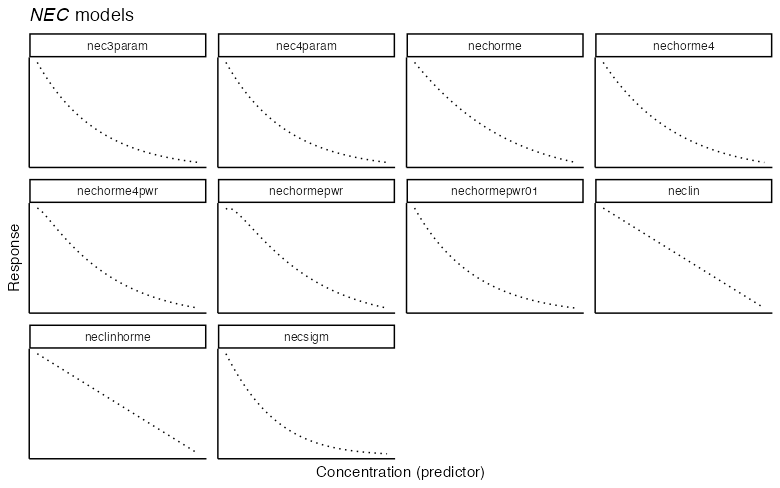
\includegraphics[width=1\textwidth]{../vignettes/vignette-fig-exmp2b-theoretical_nec_curves.png}
  \caption{Representative shapes of currently implemented \pkg{bayesnec} \textit{NEC} models.}
  \label{fig2}
\end{figure}

\hypertarget{priors-on-model-parameters}{%
\subsection{Priors on model parameters}\label{priors-on-model-parameters}}

To undertake a Bayesian analysis, prior probability densities of the parameters of the model must first be defined. Sometimes there may be substantial prior knowledge, for example when pilot data or data from a previous experiment exist for a given response curve. In this case the prior probability distribution may be quite narrow (highly ``informative'') and will therefore be influential in the characterisation of the posterior, especially when subsequent data are scarce or highly variable. However, in our experience in ecology and related disciplines, such prior knowledge is generally the exception. Where no quantitative prior information exists, it is common in Bayesian statistics to use either ``vague'' or ``weakly'' informative priors. The use of ``vague'', ``diffuse'', ``flat'' or otherwise so-called ``uninformative'' priors is no longer recommended \citep{Banner2020}. Such priors generally form the default for many Bayesian packages, and are often used in practice without critical thought or evaluation, possibly as a result of fear of being too subjective \citep{Banner2020}. However, even vague priors can have a substantial influence on the outcome of an analysis \citep{depaoli2020importance, gelman2017entropy}. Instead, it is better to use weakly informative, ``generative'' priors - that is priors that are based on probability distributions that interact sensibly with the likelihood to produce a meaningful data generating mechanism \citep{gelman2017entropy}.

Considerable thought has gone into development of an algorithm to build default ``weakly'' informative priors for fitting models in \pkg{bayesnec}. The default priors are ``weakly'' informative in that in addition to specifying the relevant statistical \code{family} that appropriately captures the parameter's theoretical statistical distribution, when external
subjective information is unavailable we also use information contained within the observed data to center the probability density of the prior within a plausible region of the parameter space, ensure priors are appropriately scaled relative to the range of the response and predictor data, and/or constrain priors to sensible bounds (described in more detail below). These weakly informative priors are used to help constrain the underlying routines so that they are less likely to consider what the researcher would deem highly improbable estimates, that may also cause the routines to become unstable resulting in failed model fits. Weakly informative priors can be particularly helpful in complex non-linear modelling to ensure reliable convergence. These types of priors specify the general shape and bounds of the probability distribution for a given parameter, whilst remaining sufficiently broad so as not to influence the parameter's estimated posterior distribution (given a reasonable amount of observed data). In this sense, appropriately weak priors should yield analytical outcomes that share the same level of \emph{objectivity} as equivalent frequentist approaches, whilst yielding robust parameter estimates with probabilistically interpretable uncertainty bounds.

While we sacrifice Bayesian coherence by using features of the data to calibrate our default priors (see \citet{chipman2010} for another example of such an approach), our primary motivation is to facilitate easy implementation of \pkg{Bayesnec} in practice, and to ensure model stability and reliable model fits. Note, however that it is critical for users to interrogate these default priors, using for example, sensitivity analysis \citep{depaoli2020importance} and ensure they are appropriate given the data \citep{gelman2017entropy}. Priors are automatically saved as part of the \code{brmsfit} and \code{bayesnecfit} models, and there are functions for extracting the priors used, as well as plotting these in comparison to the resulting posterior distribution (see Section \ref{moddiag}). Care should be taken to ensure that the default priors are sufficiently weak relative to the posterior

\hypertarget{priors-for-response-scaled-parameters}{%
\subsubsection{Priors for response-scaled parameters}\label{priors-for-response-scaled-parameters}}

Only the parameters \(\tau = \text{top}\) and \(\delta = \text{bottom}\) relate directly to the response variable's distribution. For Gaussian-distributed responses (or any response variable for which the link ensures valid values of the response can take from -\(\infty\) to \(\infty\), including \code{"log"} and \code{"logit"}) priors are Gaussian with a mean set at the 90\textsuperscript{th} and 10\textsuperscript{th} quantiles of the response for parameters \(\tau = \text{top}\) and \(\delta = \text{bottom}\), respectively, and a standard deviation of 2.5 times the standard deviation of the response (on the appropriate link scale). In this way \pkg{bayesnec} attempts to construct a prior that scales appropriately with the response data, with greatest density near the most likely region of the response for both \(\tau = \text{top}\) and \(\delta = \text{bottom}\). The priors for top and bottom can be set quite narrow and still remain relatively ``weak'' because \pkg{bayesnec} only allows models that represent an overall decrease from the start to the end of the concentration range. Because this directional relationship is pre-defined, it is reasonable to presume that the true value of \(\tau = \text{top}\), for example, should be relatively near the upper quantile of the observed response data, and a somewhat narrow prior on that assumption can be used without being strongly informative. In the context of a standard deviation across the whole response range, a value of 2.5 can still be considered relatively broad and should have little influence on the parameter's posterior density.

For Poisson-, Negative-binomial- and Gamma-distributed response variables, the response cannot take negative values and therefore Gaussian priors are unsuitable. Instead, we use Gamma priors with a mean scaled to correspond to the 75\textsuperscript{th} and 25\textsuperscript{th} quantiles of the response for \(\tau = \text{top}\) and \(\delta = \text{bottom}\), respectively. The mean (\(\mu\)) is linked mathematically to the shape (s) and rate parameters (r) by the equation \[ \mu = s * (1/r) \] \citep{Becker1988} with the shape parameter being set to 2 by default. The value of 2 was selected based on trial and error through initial testing, as this appeared to produce relatively broad priors that were still centered around feasible values for these parameters.

For the Binomial, Beta, and Beta-binomial families, estimates for \(\tau = \text{top}\) and \(\delta = \text{bottom}\) must necessarily be constrained between 0 and 1 when modelled on the identity link. Because of this constraint, there is no need to adjust scaling based on the response. In this case \pkg{bayesnec} uses \code{beta(5, 2)} and \code{beta(2, 5)} priors to provide a broad density centred across the upper and lower 0 to 1 range for the \(\tau = \text{top}\) and \(\delta = \text{bottom}\) parameters respectively.

\hypertarget{priors-for-predictor-scaled-parameters}{%
\subsubsection{Priors for predictor-scaled parameters}\label{priors-for-predictor-scaled-parameters}}

The parameters \(\eta = \text{NEC}\) and \(\omega\) = \(\text{EC\textsubscript{50}}\) scale according to the predictor variable because both of these are estimated in units of the predictor (usually concentration). To stabilise model fitting, the \(\eta = \text{NEC}\) and \(\omega\) = \(\text{EC\textsubscript{50}}\) parameters are bounded to the upper and lower observed range in the predictor, under the assumption that the range of concentrations in the experiment were sufficient to cover the full range of the response outcomes. Note that this assumption may not always hold if the data are from an experiment that is badly designed, and the outcome of any analysis resulting in either \(\eta\) or \(\omega\) being estimated at the bounds of the predictor data range should be interpreted with caution. The priors used reflect the characteristics of the observed data that are used to predict the appropriate \code{family}. If the predictor variable is strictly positive, a Gamma prior is used, with maximum density (\(\mu\), see above) at the median value of the predictor, and a shape parameter of 5. If the predictor variable is truncated at both 0 and 1, a \code{beta(2, 2)} prior is used. For predictor variables ranging from -\(\infty\) to \(\infty\), a Gaussian prior is used, with a mean set at the median of the predictor values and a standard deviation of 10 times the standard deviation of the predictor variable. A much broader prior is required for the \(\eta = \text{NEC}\) and \(\omega\) = \(\text{EC\textsubscript{50}}\) estimates than for example \(\tau = \text{top}\) and \(\delta = \text{bottom}\), because depending on the curve that is fit estimates for these parameters may fall almost anywhere along the predictor range - especially if the CR experiment was badly designed. We set the maximum density for these parameters as the median of the predictor value (in the hope that the experiment has been well designed and the inflection point is somewhere in the center of the predictor range), but it is important that there is substantial range in the prior, because the true values may be quite low or high across the predictor range, thus a very broad standard deviation of 10 is used.

\hypertarget{priors-for-other-parameters}{%
\subsubsection{Priors for other parameters}\label{priors-for-other-parameters}}

For the parameters \(\beta = \text{beta}\), \(\alpha = \text{slope}\) and \(\epsilon = \text{d}\) we first ensured any relevant transformations in the model formula such that theoretical values with the range -\(\infty\) to \(\infty\) are allowable, and a \code{normal(0, 5)} (mean and standard deviation) prior is used. For example in the \code{nec3param} model, \(\beta = \text{beta}\) is an exponential decay parameter, which must by definition be bounded to 0 and \(\infty\). Calling \code{exp(beta)} in the model formula ensures the exponent meets these requirements. Note also that a mean of 0 and standard deviation of 5 represents a relatively broad prior on this exponential scaling, so this is usually a weakly informative prior in practice.

\subsubsection[User-specified priors]{User-specified priors}\label{usp}

In \pkg{bayesnec} we chose to provide default weakly informative priors that are scaled according to the characteristics of the input data (discussed in detail above) in some cases. They were designed to be somewhat informative (relative to each parameter's region) but that would, in data-sufficient cases, return fits without HMC divergent transitions in \proglang{Stan}. Default ``blanket'' priors are not currently provided for non-linear models by the model-building underlying package \pkg{brms}, and we note that defining the extent to which a prior is vague or weakly/strongly informative ultimately depends on the likelihood \citep{gelman2017entropy}. Therefore, there may be situations where the default \pkg{bayesnec} priors do not behave as desired, or the user wants to provide customised priors. For example, the default priors may be too informative, yielding unreasonably tight confidence bands (although this is only likely where there are few data or unique values of the predictor variable). Conversely, priors may be too vague, leading to poor model convergence. Alternatively, the default priors may be of the wrong statistical \code{family} if there was insufficient information in the provided data for \pkg{bayesnec} to correctly predict the appropriate ones to use. The priors used in the default model fit can be extracted using \code{pull_prior}, and a sample or plot of prior values can be obtained from the individual \pkg{brms} model fits through the function \code{sample_priors} which samples directly from the \code{prior} element in the \code{brmsfit} object (\code{pull_brmsfit(fit) |> prior_summary() |> sample_priors()}, see \autoref{fig:sampleprior}). We show example usage of these functions under the Section \ref{moddiag} below.

\subsection[Model averaging]{Model averaging}\label{modavg}

Multi-model inference can be useful where there is a range of plausible models that could be used \citep{Burnham2002} and has been recently adopted in ecotoxicology for Species Sensitivity Distribution (SSD) model inference \citep{Thorley2018, fox2020, Dalgarno}. The approach may have considerable value in CR modelling because there is often no a priori knowledge of the functional form that the response relationship should take. In this case, model averaging can be a useful way of allowing the data to drive the model selection process, with weights proportional to how well the individual models fit the data. Well-fitting models will have high weights, dominating the model averaged outcome. Conversely, poorly fitting models will have very low model weights and will therefore have little influence on the outcome. Where multiple models fit the data equally well, these can equally influence the outcome, and the resultant posterior predictions reflect that model uncertainty.

\pkg{bayesnec} adopts the weighting methods implemented in the \pkg{loo} \citep{vehtari2020} package in \proglang{R}. \pkg{loo} provides an efficient approximate leave-one-out cross-validation (LOO) algorithm for Bayesian models fit using Markov chain Monte Carlo, as described in \citep{vehtari2017} \url{doi:10.1007/s11222-016-9696-4}. The approximation uses Pareto smoothed importance sampling (PSIS), a new procedure for regularizing importance weights and follows the implementation described in \citep{Vehtari2019}. The \pkg{loo} package offers two weighting methods, the \code{"stacking"} method, aimed to minimise prediction error \citep{Yao2018}, and the \code{"pseudobma"} method, with and without Bayesian bootstrap \citep{vehtari2020, vehtari2017}. The stacking method (\code{method = "stacking"}), combines all models by maximizing the leave-one-out predictive density of the combination distribution, such that it finds the optimal linear combining weights for maximizing the leave-one-out log score \citep{vehtari2020}. The pseudo-BMA method (\code{method = "pseudobma"}) finds the relative weights proportional to the theoretical expected log pointwise predictive density of each model \citep{vehtari2020}. The Bayesian bootstrap (when using \code{method = "pseudobma"}) takes into account the uncertainty of finite data points and regularizes the weights away from the extremes of 0 and 1 \citep{vehtari2020}. \pkg{bayesnec} currently uses by default the \code{"pseudobma"} method (\code{method = "pseudobma"}) with Bayesian bootstrap (\code{BB = TRUE}), but this can be easily modified via argument \code{loo_controls}.

\hypertarget{usage}{%
\section{Usage}\label{usage}}

\subsection[The fitting function bnec]{The fitting function \emph{bnec}}\label{ffbnec}

The main working function in \pkg{bayesnec} is \code{bnec}. We have attempted to make the \code{bnec} function as easy to use as possible, targeting the \proglang{R} user that is familiar with the usual model fitting syntax in \proglang{R}, but without specialist expertise in non-linear modelling and Bayesian statistics. We can run \code{bnec} by supplying the argument \code{formula}: a special custom formula which comprises the relationship between response and predictor, and the CR model (or models) chosen to be fitted; and \code{data}: a \code{data.frame} containing the data for the model fitting.

\hypertarget{the-input-formula}{%
\subsection{The input formula}\label{the-input-formula}}

In its simplest syntax, the basic \code{bnec} formula should be of the form:

\begin{CodeChunk}
\begin{CodeInput}
R> response ~ crf(predictor, model = "a_model")
\end{CodeInput}
\end{CodeChunk}

where the left-hand side of the formula is implemented exactly as in \pkg{brms} (see the `aterms' Section of the \code{brms::brm}'s help file). The right-hand side of the formula contains the special internal function \code{crf} (which stands for concentration-response function), and takes the predictor (including any simple function transformations such as \code{"log"}) and the desired CR model or suite of models. As with any formula in \proglang{R}, the name of the terms need to be exactly as they are in the input data.frame. For Binomial- or Beta-Binomial distributed data, the user needs to include the \code{trials} term to the left-hand side of the formula, e.g.

\begin{CodeChunk}
\begin{CodeInput}
R> response | trials(n_trials) ~ crf(log(predictor), model = "a_model")
\end{CodeInput}
\end{CodeChunk}

The input formula can either be a character string or a validated object of class \code{bayesnecformula}. Details about existing possibilities are detailed in the help files of \code{bayesnecformula} and \code{check_formula}. The argument \code{model} in the formula function \code{crf} is a character string indicating the name(s) of the desired model(s). Alternatively, it may also be one of \code{"all"}, meaning all of the available models will be fit; \code{"ecx"} meaning only models excluding the \(\eta = \text{NEC}\) step parameter will be fit; \code{"nec"} meaning only models with a specific \(\eta = \text{NEC}\) step parameter will be fit; \code{"bot_free"} meaning only models without a \(\delta\) (\code{bottom, "bot"}) parameter (without a lower plateau) will be fit; \code{"zero_bounded"} are models that are bounded to be zero; or \code{"decline"} excludes all hormesis models, i.e., only allows a strict decline in response across the whole predictor range (see above Section \ref{mdbnc}).

The class \code{bayesnecformula} (generated by the function \code{bayesnecformula} and its alias \code{"bnf"}) contains a \code{model.frame} method which can be employed to manually inspect the \code{data.frame} that will be used to run checks on the data suitability prior to model fitting, e.g.

\begin{CodeChunk}
\begin{CodeInput}
R> library("bayesnec")
R> set.seed(17)
R> df <- data.frame(x = rgamma(100, 2, 0.1), y = rnorm(100))
R> form <- bnf(y ~ crf(log(x), model = "nec3param"))
R> head(model.frame(form, df))
\end{CodeInput}
\begin{CodeOutput}
            y   log(x)
1  1.93723559 1.637897
2 -0.50355786 3.249447
3  0.09236529 2.786040
4  1.06937160 1.806777
5 -0.48396058 2.568040
6 -0.41780030 3.366183
\end{CodeOutput}
\end{CodeChunk}

\subsection[Example]{Example}\label{example}

Here we use one of the package's built-in data sets, \code{"nec_data"}, which is a simulated data set based on the three parameter NEC model \code{nec3param} described in Section \ref{mdbnc}.

\begin{CodeChunk}
\begin{CodeInput}
R> fit <- bnec(y ~ crf(x, model = "nec3param"), data = nec_data,
+             seed = 17)
\end{CodeInput}
\end{CodeChunk}

If a recognized model name is provided, a single model of the specified type is fit, and \code{bnec} returns an object of class \code{bayesnecfit}. If a vector of two or more of the available models are supplied, or if one of the model-sets is specified, \code{bnec} returns a model object of class \code{bayesmanecfit} containing Bayesian model averaged predictions for the supplied models, providing they were successfully fitted (see \ref{modavg} above, and the help file of \code{bnec} for further details). By default, \code{bnec} sets the number of chains to 4, the number of iterations per chain to 10,000, and the size of the warm-up period to 4/5 of the number of iterations (i.e 8,000 by default).

\code{bnec} will guess the most likely distribution for the response variable. This ``guess'' is achieved through the internal function \code{set_distribution}. This algorithm will assume a Binomial distribution for the response if data are integers and \code{trials(...)} is passed in the formula call; Poisson if data are integers and there are no \code{trials(...)}; Gamma if the data are continuous, zero bounded and contain values greater than one; Beta if data are continuous and bounded to zero and one; and Gaussian if data are continuous and contain negative values. The \code{family} can be set manually via the usual \proglang{R} syntax of calling the argument \code{family} and specifying the desired distribution. \pkg{bayesnec} currently supports the use of the above listed families, as well as the Negative-Binomial and Beta-binomial families that can be used in the case of over-dispersed Binomial and Poisson families respectively.

In the example here, the model was fitted assuming a Beta distribution on an identity link because the response is truncated at both 0 and 1 and contains decimal values. Note that the default behaviour in \pkg{bayesnec} is to use the \code{"identity"} link because the native link functions for each \code{family} (e.g., \code{"logit"} for Binomial, \code{"log"} for Poisson) introduce non-linear transformation on formulas which are already non-linear. So please be aware that estimates of ECx might not be as expected when using link functions other than identity. Additionally, \code{bnec} will also generate appropriate priors for the internal \code{brms::brm} model call. However, \code{bnec} allows the user to pass additional arguments to \code{brms::brm} and therefore the user can, for example, manually add specific distributions and link functions via the argument \code{family}, or custom priors via the argument \code{prior}. Please refer to the rich set of resources available for the \pkg{brms} package at \url{https://github.com/paul-buerkner/brms} for further information.

\hypertarget{output-classes-and-methods}{%
\subsection{Output classes and methods}\label{output-classes-and-methods}}

Models fitted by \code{bnec} will invariably inherit a class \code{bnecfit} which carries three exclusive methods: \code{+}, \code{c} and \code{update}. The first two are used to append one or multiple models to an existing fit, whereas the latter is used to update the fitting characteristics of an existing model (e.g., change the number of iterations or warm-up period, or simply change the HMC fitting parameters).

When \code{bnec} fits a single CR model type, the output object also inherits the \code{bayesnecfit} class. This class contains the \code{brmsfit} object in addition to the mean predicted values and summary estimates of each model parameter. Because the original motivation in the development of \pkg{bayesnec} was the estimation of no-effect toxicity values, by default \code{bnec} also returns a full posterior distribution of the either the NEC (for \textbf{nec} models) or the NSEC (for \textbf{ecx} models, see \citet{Fisher2023}) estimate. If \code{bnec} fits a custom set of models, or a package-pre-defined model-set (e.g.~\code{model = "decline"} in the input formula), the output object is going to inherit the \code{bayesmanecfit} class. Differently from a \code{bayesnecfit} object, \code{bayesmanecfit} comprises a model weighted estimate of predicted posterior values of N(S)EC. This is a weighted combined average of the NEC or the NSEC values, for all \textbf{nec} and \textbf{ecx} models respectively, as described in \citet{fisher2023ieam}.

Regardless of if \code{bnec} generates a \code{bayesnecfit} or \code{bayesmanecfit} class, the underlying \code{brmsfit} object can be extracted using the function \code{pull_brmsfit}. The \code{brmsfit} contains all of the information usually returned from a call to \code{brm}, including the posterior samples of all parameters in the model, from which predictions can be made and custom probabilities calculated.

Both \code{bayesnecfit} and \code{bayesmanecfit} classes contain methods for \code{summary}, \code{print}, \code{predict}, \code{model.frame}, \code{fitted}, \code{posterior_predict}, \code{posterior_edpred} and plotting (\code{plot} and \newline \code{autoplot}). Wherever possible, these methods have been implemented such they are consistent with other model fitting packages in \proglang{R}, and in particular \pkg{brms}. We have also implemented a range of custom functions for extracting effect concentrations and related threshold values (\code{nec}, \code{ecx} and \code{nsec}) that, in the case of a \code{bayesmanecfit}, return model weighted estimates.

The \code{summary} method provides the usual summary of model parameters and any relevant model fit statistics as returned in the underlying \code{brm} model fit(s). In the specific case of a \code{bayesmanecfit} object, the summary includes a list of fitted models, their respective model weights, and a model-averaged NEC---which is reported with a warning when it contains NSEC values (see below Section \ref{modsuit}).

\begin{CodeChunk}
\begin{CodeInput}
R> summary(fit)
\end{CodeInput}
\begin{CodeOutput}
Object of class bayesnecfit containing the following non-linear model: nec3param

 Family: beta 
  Links: mu = identity; phi = identity 
Formula: y ~ top * exp(-exp(beta) * (x - nec) * step(x - nec)) 
         top ~ 1
         beta ~ 1
         nec ~ 1
   Data: data (Number of observations: 100) 
  Draws: 4 chains, each with iter = 10000; warmup = 8000; thin = 1;
         total post-warmup draws = 8000

Population-Level Effects: 
     Estimate Est.Error l-95% CI u-95% CI Rhat Bulk_ESS Tail_ESS
top      0.89      0.01     0.88     0.90 1.00     6743     5367
beta     0.54      0.06     0.42     0.66 1.00     5522     5291
nec      1.54      0.02     1.50     1.57 1.00     5228     4596

Family Specific Parameters: 
    Estimate Est.Error l-95% CI u-95% CI Rhat Bulk_ESS Tail_ESS
phi    51.70      7.48    38.91    68.56 1.00     7020     5598

Draws were sampled using sampling(NUTS). For each parameter, Bulk_ESS
and Tail_ESS are effective sample size measures, and Rhat is the potential
scale reduction factor on split chains (at convergence, Rhat = 1).


Bayesian R2 estimates:
   Estimate Est.Error Q2.5 Q97.5
R2     0.96      0.00 0.96  0.97
\end{CodeOutput}
\end{CodeChunk}

As mentioned above, the visualization of a particular model fit can be done via either \pkg{base} \proglang{R} (\code{plot}) and \pkg{ggplot2} \citep{ggplot} (\code{autoplot}). Here we pass the additional argument \code{xform} which ensures that the NEC estimate is transformed to the proper scale (because the original formula contained \code{log(concentration)}):

\begin{CodeChunk}
\begin{CodeInput}
R> round_digits <- function(x) sprintf("%.2f", x)
R> autoplot(fit, xform = exp) +
+   scale_x_continuous(trans = "log", labels = round_digits)
\end{CodeInput}
\begin{figure}[!ht]

{\centering \includegraphics{article_files/figure-latex/base-plot-1} 

}

\caption{\pkg{ggplot2} \code{autoplot} of the example fit. The solid black line is the fitted median of the posterior prediction, dashed black lines are the 95\% credible intervals, and the vertical lines show the estimated \textit{NEC} value.}\label{fig:base-plot}
\end{figure}
\end{CodeChunk}

By default the plot shows the fitted posterior curve with 95\% credible intervals, along with an estimate of the \(\eta = \text{NEC}\) value. Please see on-line the vignettes at \url{https://open-aims.github.io/bayesnec/articles/} for more examples using \pkg{bayesnec} models for inference, as well as Section \ref{modsuit} below.

\subsection[Model diagnostics]{Model diagnostics}\label{moddiag}

\pkg{bayesnec} will return warning messages as part of the summary method where parts of the model have not converged (rhat, \(\widehat{R}\) \textgreater{} 1.05, see \citet{vehtari2021rank}) and indicate the number of any divergent transitions (if any). These messages include guidance on running more iterations, adjusting priors and or adjusting other fitting criteria, such as adapt\_delta. The summary method for a \code{bayesnecfit} object also indicates the effect sample size for estimates of each of the parameters, and for a \code{bayesmanecfit} a warning is returned if any of the models have parameters with an effective sample size of \textless100.

In addition to the diagnostic information reported by the summary method, a range of tools is available to assess model fit, including an estimate of overdispersion (for relevant families), an extension of the \pkg{brms} \code{rhat} function that can be applied to both \code{bayesnecfit} and \code{bayesmanecfit} model objects, and a function \code{check_chains} that can be used to visually assess chain mixing and stability.

All diagnostic functions available in \pkg{brms} and \pkg{rstan} can be used on the underlying \code{brm} model fit by extracting the fitted \pkg{brms} model from the \code{bayenecfit} or \code{bayesmanecfit} model object using the function \code{pull_brmsfit}. For example, we can use the default \pkg{brms} plotting method to obtain a diagnostic plot of the individual fit of the \code{nec4param} model using:

\begin{CodeChunk}
\begin{CodeInput}
R> brms_fit <- pull_brmsfit(fit)
R> plot(brms_fit)
\end{CodeInput}
\begin{figure}[!ht]

{\centering \includegraphics{article_files/figure-latex/brmsplot-1} 

}

\caption[Default \pkg{brms} plot of the \code{nec3param} model showing the posterior densities and chain mixing for each of the included parameters]{Default \pkg{brms} plot of the \code{nec3param} model showing the posterior densities and chain mixing for each of the included parameters.}\label{fig:brmsplot}
\end{figure}
\end{CodeChunk}

which yields a plot of the posterior densities as well as trace plots of chains for each parameter in the specified model (\autoref{fig:brmsplot}).

Several helper functions have been included that allow the user to add or drop models from a \code{bayesmanecfit} object, or change the model weighting method (\code{amend}); extract a single or subset of models from the \code{bayesmanecfit} object (\code{pull_out}); and examine the priors used for model fitting (\code{pull_prior}, \code{sample_priors} and \code{check_priors}).

The priors used in the default model fit can be extracted using \code{pull_prior}, and a sample or plot of prior values can be obtained from the individual \pkg{brms} model fits through the function \code{sample_priors} which samples directly from the \code{prior} element in the \code{brmsfit} object (\code{pull_brmsfit(fit) |> prior_summary() |> sample_priors()}, see \autoref{fig:sampleprior}).

\begin{CodeChunk}
\begin{figure}[!ht]

{\centering \includegraphics{article_files/figure-latex/sampleprior-1} 

}

\caption[Frequency histograms of samples of the default priors used by \pkg{bayesnec} for fitting the \code{nec3param} model to the example data]{Frequency histograms of samples of the default priors used by \pkg{bayesnec} for fitting the \code{nec3param} model to the example data.}\label{fig:sampleprior}
\end{figure}
\end{CodeChunk}

We can also use the function \code{check_priors} (based on the \code{hypothesis} function of \pkg{brms}) to assess how the posterior probability density for each parameter differs from that of the prior. Here we show the prior and posterior probability densities for the parameters in the \texttt{nec4param} model fit (\texttt{check\_priors(fit)}, see \autoref{fig:checkpriorsingle}). There is also a \code{bayesmanecfit}-specific method that can be used to sequentially view all plots in a \code{bnec} call with multiple models, or write to a pdf as in \code{check_chains}.

\begin{CodeChunk}
\begin{figure}[!ht]

{\centering \includegraphics{article_files/figure-latex/checkpriorsingle-1} 

}

\caption[A comparison of the prior and posterior parameter probability densities for the \code{nec3param} model fit to the example data]{A comparison of the prior and posterior parameter probability densities for the \code{nec3param} model fit to the example data.}\label{fig:checkpriorsingle}
\end{figure}
\end{CodeChunk}

\hypertarget{model-comparison}{%
\subsection{Model comparison}\label{model-comparison}}

With \pkg{bayesnec} we have included a function (\texttt{compare\_posterior}) that allows bootstrapped comparisons of posterior predictions. This function allows the user to fit several different \code{bnec} model fits and compare differences in their posterior predictions. Comparisons can be made across the model fits for individual threshold estimates (e.g.~NEC, NSEC or ECx) or across a range of predictor values. Usage is demonstrated in the relevant vignette at \url{https://open-aims.github.io/bayesnec/articles/example4.html} by comparing different types of models and model-sets using a single data set. However, the intent of this function is to allow comparison across different data sets that might represent, for example, different levels of a fixed factor covariate. For example, this function has been used to compare toxicity of herbicides across three different climate scenarios, to examine the cumulative impacts of pesticides and global warming on corals \citep{flores2021}.

At this time \code{bnec} does not allow for an inclusion of an interaction with a fixed factor. Including an interaction term within each of the non-linear models implemented in \pkg{bayesnec} is relatively straightforward, and may be introduced in future releases. However, in many cases the functional form of the response may change with different levels of a given factor. The substantial complexity of defining all possible non-linear model combinations at each factor level means it unlikely this could be feasibly implemented in \pkg{bayesnec} in the short term. In the meantime the greatest flexibility in the functional form of individual model fits can be readily obtained using models fitted independently to data within each factor level.

\hypertarget{hierarchical-effects}{%
\subsection{Hierarchical effects}\label{hierarchical-effects}}

Most ecotoxicological and toxicology experiments include a range of grouping elements, such as tanks, vials or batches of samples that contain multiple measurements that cannot be considered strictly independent (a.k.a. they are pseudo-replicates). To avoid criticism around potential issues with pseudo-replication, it is often the practice for ecotoxicologists to pool such observations and carry out modelling using, for example, the group mean. Where the number of within group observations varies substantially across groups, this will have the undesirable effect of equally weighting the group means even though some may be based on far fewer observations than others. In addition, there are often instances of ecotoxicology data from multiple experiments or other grouping factors within an experiment (such as genotype) that cover the full range of the predictor variable that cannot be averaged prior to modelling, resulting in the ecotoxicologist either ignoring the potential non-independence, or fitting many independent data sets and subsequently needing to aggregate the threshold estimates. Carrying out multiple fits on separate data sets is undesirable because each fit is based on fewer data and will have greater uncertainty.

The current version of \pkg{bayesnec} harnesses the powerful modelling flexibility of \pkg{brms} for accommodating hierarchical designs and other forms of non-independence. This is achieved by allowing a list of grouping terms to be added to a \code{bayesnecformula}, which are then used to generate the underlying \code{brmsformula} for the \pkg{brms} internal call. Hierarchical effects can be in the form of an offset, which effectively allows different mean response levels across groups, and is achieved by specifying the \texttt{ogl} (offset group-level) formula term. Hierarchical effects can also be added to any or all of the (non-)linear parameters in the model by specifying the \texttt{pgl} (parameter group-level) formula term. Note that implementing hierarchical effects in a non-linear modelling setting is non-trivial and considerable thought and testing should go into selecting an appropriate hierarchical structure, and potentially suitable priors. Examples of how to implement hierarchical effects in \pkg{bayesnec} can be found on the help file of function \code{"bnf"}.

\section[Existing alternatives]{Existing alternatives}\label{bnchmrk}

\pkg{bayesnec} is built upon the precursor \proglang{R} package \pkg{jagsNEC} \citep{fisher2020}, which writes and fits CR models in \proglang{JAGS} \citep{Plummer2003}. \pkg{bayesnec} was then expanded to include several additional CR models and further generalised to allow a large range of response variables to be modelled using their appropriate statistical distribution. In addition, \pkg{bayesnec} allows the addition of hierarchical effects (see above). The simpler syntax of \pkg{brms} allows \pkg{bayesnec} to be more easily expanded to include additional response distributions as well as CR model formula. In addition, \pkg{brms} is well developed and comes with a large range of supporting functions not available to the \proglang{jags} equivalents.

While there are some commercial propriety software packages to support the analysis of toxicity data, such as graphpad (\url{https://www.graphpad.com}) and ToxCalc (\url{https://www.tidepool-scientific.com/ToxCalc/ToxCalc.html}), these provide limited flexibility and most importantly do not support fully reproducible analysis in an open-source environment. Ensuring that the raw data from the experiment are available; and that the statistical code and documentation to reproduce the analysis are also available are two major components to a reproducible study \citep{peng2015}.

The open-source flexible computing environment \proglang{R}, provides an ideal platform for reproducible analysis of toxicity data sets. The main existing tool in \proglang{R} that is widely used in ecotoxicology and toxicology is the frequentist-based package \pkg{drc} \citep{Ritz2016}. \pkg{drc} provides a suite of flexible and versatile model fitting and after-fitting functions for the analysis of dose-response data. The package includes a large range of built-in dose-reponse models that are parameterized using a unified structure with a coefficient b denoting the steepness of the dose-response curve (\(\beta = \text{beta}\) in \pkg{bayesnec}); c and d the lower and upper asymptotic limits of the response (\(\tau = \text{top}\) and \(\delta = \text{bottom}\) in \pkg{bayesnec}); and, for some models, e the effective dose ED50 (\(\omega\) = \(\text{EC\textsubscript{50}}\) in \pkg{bayesnec}) \citep{Ritz2016}. Estimation in \pkg{drc} is based on the maximum likelihood principle, which under the assumption of normally distributed response values simplifies to nonlinear least squares. \pkg{bayesnec} provides a Bayesian implementation of many of the non-linear models offered by \pkg{drc}.

We compared the \pkg{drc} and \pkg{bayesnec} fits for the three parameter no-effect-concentration model implemented in WinBugs by \citet{Fox2010} (the \code{nec3param} model in \pkg{bayesnec}, see Section \ref{nec-models}) for two selected herbicides from the data from \citet{jones2003meps}. The data comprise assays of herbicide phytotoxicity on chlorophyll fluorescence measurements (Fv/Fm) of symbiotic dinoflagellates still in the host tissue of the coral. Full detail on this example data set is provided in Section \ref{iexample}. In \pkg{bayesnec} this model is fit with the call \texttt{bnec(fvfm\ \textasciitilde{}\ crf(log\_x,\ model\ =\ "nec3param"),\ data\ =\ .x)}, and in \pkg{drc} using \texttt{drm(fvfm\ \textasciitilde{}\ log\_x,\ fct\ =\ NEC.3(),\ data\ =\ .x)}. The herbicides hexazinone and tebuthiuron were selected specifically for this comparison as visual inspection indicated they should provide a reasonable fit to the \citet{Fox2010} model as there was some evidence of a threshold effect. For both herbicides, the predicted \pkg{drc} and \pkg{bayesnec} values were nearly identical using the default behaviour of each package (\autoref{fig:drccomparisonplot}).

\begin{CodeChunk}
\begin{figure}[!ht]

{\centering \includegraphics{article_files/figure-latex/drccomparisonplot-1} 

}

\caption[A comparison of the \pkg{bayesnec} and \pkg{drc} model fits and estimated NEC values for the \code{nec3param} model, fit to data on maximum effective quantum yield ($\Delta F / Fm'$) of symbiotic dinoflagellates (in hospite) in \textit{Seriatopora hystrix} exposed to elevated hexazinone and tebuthiuron (range 0.3 to 1000 ug per L) for 10 h]{A comparison of the \pkg{bayesnec} and \pkg{drc} model fits and estimated NEC values for the \code{nec3param} model, fit to data on maximum effective quantum yield ($\Delta F / Fm'$) of symbiotic dinoflagellates (in hospite) in \textit{Seriatopora hystrix} exposed to elevated hexazinone and tebuthiuron (range 0.3 to 1000 ug per L) for 10 h.}\label{fig:drccomparisonplot}
\end{figure}
\end{CodeChunk}

While \pkg{drc} is an excellent tool for fitting CR models using frequentist methods and is widely used (\citet{Ritz2016} currently has nearly 2,000 citations), \pkg{bayesnec} provides a Bayesian alternative using similarly simple syntax. The advantages of Bayesian methods in this setting are numerous, and include direct characterisation of parameter uncertainty and posterior predicted samples that provide a valuable resource for model inference (such as comparisons of relative toxicity, see Section \ref{iexample} and \autoref{fig:necplots}). In addition, we have observed that even the use of only weakly informative priors tends to improve the reliability of model fits compared to \pkg{drc}, and this may be true of MLE estimation more generally \citep{krull2020comparing}.

\section[Illustrative example]{Illustrative example}\label{iexample}

So far we have demonstrated the basic usage of \pkg{bayesnec} and compared the results for a single model fit to \pkg{drc}. Here we work through an illustrative example demonstrating the use of the package for a data set on herbicide toxicity. The aim here is to indicate the usual workflow and highlight the advantages of model averaging combined with Bayesian methods as a rigorous means of estimating and comparing relative toxicity, and the associated uncertainty. The data we analyse in this example are from \citet{jones2003meps}.

\hypertarget{example-case-study}{%
\subsection{Example case study}\label{example-case-study}}

In our case study, the no-effect-toxicity values of a range of herbicides are first estimated and then their relative toxicity is compared. The response data are the maximum effective quantum yield (\({\Delta F / Fm'}\)) of symbiotic dinoflagellates still in the host tissue of the coral \emph{Seriatopora hystrix} (in hospite or in vivo). \({\Delta F / Fm'}\) was calculated from Chlorophyll fluorescence parameters measured using a DIVING-PAM chlorophyll fluorometer (Walz) as described in more detail in \citet{jones2003meps} and \citet{jones2003effects}. The corals were exposed to elevated levels of eight different herbicides (Irgarol 1051, ametryn, diuron, hexazinone, atrazine, simazine, tebuthiuron, ioxynil) at concentrations ranging from 0.3 to 1000 \({\mu g/L}\)) for 10 h. Data for ioxynil were excluded from analysis here as this herbicide did not show sufficient response at the maximum concentration.

\subsection[Single herbicide]{Single herbicide analysis}\label{isingle}

We start by describing the analysis workflow for a single herbicide, ametryn. We first filter ametryn from the larger herbicide data set. The concentration data are log transformed prior to analysis to improve model stability and because this is the natural scaling of the concentration series for these data. As there was little evidence of hormesis (an initial increase in the response at low concentration) in these data (or in the other herbicides, see below \ref{iall}), we used only the \code{decline} model set as candidate models for the model averaging. Setting \code{model = "decline"} results in \pkg{bayesnec} attempting to fit a set of 14 models, and returning an object of class \texttt{bayesmancfit} for the herbicide ametryn.

\begin{CodeChunk}
\begin{CodeInput}
R> ametryn <- herbicide |>
+   dplyr::mutate(concentration = log(concentration)) |> 
+   dplyr::filter(herbicide == "ametryn")
R> manecfit_ametryn <- bayesnec::bnec(
+   fvfm ~ crf(concentration, model = "decline"), data = ametryn, seed = 17
+ )
\end{CodeInput}
\end{CodeChunk}

Other than selecting a model set to use, here we leave all other \code{bnec} arguments as their default. In this case \pkg{bayesnec} correctly chooses a Beta distribution to use as the \code{family}, defaults to the identity link, and drops the models ``neclin'' and ``ecxlin'' from the complete list of ``decline'' models (as these are not appropriate for a zero bounded distribution, such as the Beta distribution, \ref{mdbnc}). Note that in this example (or the one below, \ref{iall}) we do not show all of the console output and messages generated by both the \code{bnec} and underlying \code{brm} functions, because across 14 models this results in substantial output.

Following model fitting, the quality of the fits should be examined using the function \code{check_chains}, as well as \code{check_priors} to ensure there is good chain mixing and that the default priors were suitable. The results from these checks are omitted here for brevity, but can be easily saved to pdf output for visual inspection and inclusion into any analysis supplementary material by setting the argument \texttt{filename} to any non empty string, as in the code below:

\begin{CodeChunk}
\begin{CodeInput}
R> check_chains(manecfit_ametryn, filename = "ametryn_check_chains")
R> check_priors(manecfit_ametryn, filename = "ametryn_check_priors")
\end{CodeInput}
\end{CodeChunk}

We can also check the \code{rhat} values of the fitted models using the \code{rhat} function, based on the method of \citet{vehtari2021rank}:

\begin{CodeChunk}
\begin{CodeInput}
R> rhat(manecfit_ametryn)
\end{CodeInput}
\end{CodeChunk}

Once we are happy with the model fits, we can examine the model statistics using \code{summary}:

\begin{CodeChunk}
\begin{CodeInput}
R> summary(manecfit_ametryn)
\end{CodeInput}
\begin{CodeOutput}
Object of class bayesmanecfit

 Family: beta  
  Links: mu = identity; phi = identity  

Number of posterior draws per model:  8000

Model weights (Method: pseudobma_bb_weights):
             waic   wi
nec3param -450.82 0.02
nec4param -456.73 0.03
ecxexp    -320.61 0.00
ecx4param -465.14 0.31
ecxwb1    -443.58 0.01
ecxwb2    -461.34 0.08
ecxwb1p3  -323.30 0.00
ecxwb2p3  -446.94 0.02
ecxll5    -464.45 0.24
ecxll4    -465.06 0.30
ecxll3    -432.18 0.00


Summary of weighted NEC posterior estimates:
NB: Model set contains the ECX models: ecxexp;ecx4param;ecxwb1;ecxwb2;ecxwb1p3;ecxwb2p3;ecxll5;ecxll4;ecxll3; weighted NEC estimates include NSEC surrogates for NEC
    Estimate  Q2.5 Q97.5
NEC    -1.59 -2.09 -0.47


Bayesian R2 estimates:
          Estimate Est.Error Q2.5 Q97.5
nec3param     0.99      0.00 0.99  0.99
nec4param     0.99      0.00 0.99  0.99
ecxexp        0.89      0.01 0.87  0.91
ecx4param     0.99      0.00 0.99  0.99
ecxwb1        0.99      0.00 0.98  0.99
ecxwb2        0.99      0.00 0.99  0.99
ecxwb1p3      0.94      0.01 0.90  0.96
ecxwb2p3      0.99      0.00 0.99  0.99
ecxll5        0.99      0.00 0.99  0.99
ecxll4        0.99      0.00 0.99  0.99
ecxll3        0.99      0.00 0.98  0.99
\end{CodeOutput}
\end{CodeChunk}

For a \code{bayesmanecfit} object with multiple model fits, \code{summary} first displays the class, the \code{family} and links that have been used for the model fits, the number of posterior draws contained within each model fit, and a table of the model weights for each model, showing the Widely Applicable Information Criterion (waic, \citet{watanabe2010asymptotic}) from \pkg{loo} and weights (wi) which are based by default on the \code{"pseudobma"} method (\code{method = "pseudobma"}) with Bayesian bootstrap (\code{BB = TRUE}) (see above), but this can be easily modified via argument \code{loo_controls} using \code{amend}. For the amatryn data set, weights are highest for the \textbf{ecx4param} model, followed closely by tge \textbf{ecxll4} model, with some lesser support for the \code{ecxwb2} model, and very a small amount of support for the two \emph{NEC} models (\emph{nec3param} and \emph{nec4parm}).

Because \pkg{bayesnec} was primarily developed for estimating no-effect-concentrations, an estimate of model averaged NEC is also provided, in this case with a note that the weighted model averaged estimate contains NSEC \citep{Fisher2023} values in the case of the fitted \emph{ECx} models. In units of log concentration, the estimated no-effect toxicity value for ametryn is -1.59, which is equivalent to 0.204 \({\mu}gL^{-1}\). The 95\% credible intervals are also provided, based on the 0.025 and 97.5 quantiles of the weighted pooled posterior sample.

Finally, Bayesian \(R^2\) estimates are also provided \citep{gelman2019}, as an indicator of overall model fit. This is useful because model weights are always relative to the models actually included in the model set for the given data. The \(R^2\) provides an indicator of model fit that can be compared objectively across data sets as an indication of the quality of the fit of any of the supplied models to the data.

We can plot all the models contained within the \code{bayesmanecfit} using the \texttt{autplot} function, with all\_models = TRUE (\autoref{fig:fullbayesmanecplotametrynALLplot}):

\begin{CodeChunk}
\begin{CodeInput}
R> ametryn_plot_all <- autoplot(manecfit_ametryn, all_models = TRUE)
\end{CodeInput}
\end{CodeChunk}

We can also plot the model averaged fit that is used to derive the model averaged no-effect-concentration for ametryn, as displayed in the summary (\autoref{fig:fullbayesmanecplotametrynplot}):

\begin{CodeChunk}
\begin{CodeInput}
R> ametryn_plot <- autoplot(manecfit_ametryn)
\end{CodeInput}
\end{CodeChunk}

\begin{CodeChunk}
\begin{figure}[!ht]

{\centering \includegraphics{article_files/figure-latex/fullbayesmanecplotametrynALLplot-1} 

}

\caption{Individual model fits to the ametryn data set, showing the estimated no effect concentration for each. Data are the maximum effective quantum yield ($\Delta F / Fm'$) of symbiotic dinoflagellates (in hospite) in \textit{Seriatopora hystrix} exposed to elevated ametryn (range 0.3 to 1000 ug per L) for 10 h. N(S)EC values presented are the median and 95\% credible intervals of the posterior estimates of the NEC parameter obtained for all \code{NEC} models, and the posterior predicted NSEC values estimated from all smooth \code{ECx} models.}\label{fig:fullbayesmanecplotametrynALLplot}
\end{figure}
\end{CodeChunk}

\begin{CodeChunk}
\begin{figure}[!ht]

{\centering \includegraphics{article_files/figure-latex/fullbayesmanecplotametrynplot-1} 

}

\caption{Full model averaged bayesmanecfit to the ametryn data set, showing the estimated model-averaged no effect concentration. Data are the maximum effective quantum yield ($\Delta F / Fm'$) of symbiotic dinoflagellates (in hospite) in \textit{Seriatopora hystrix} exposed to elevated ametryn (range 0.3 to 1000 ug per L) for 10 h. N(S)EC values presented are model averaged posterior densities of the NEC parameter obtained from all fitted \code{NEC} models, and the NSEC values estimated from all smooth \code{ECx} models, summarised as a median and 95\% credible intervals. Only the \code{decline} model set was used (ie. hormesis models were excluded).}\label{fig:fullbayesmanecplotametrynplot}
\end{figure}
\end{CodeChunk}

\subsection[Comparing toxicity]{Comparing toxicity across herbicides}\label{iall}

Above we describe the workflow for a single herbicide. We now show how to use the same workflow across all herbicides to generate full \code{bayesmanecfit} model averaged fits and no-effect-toxicity estimates, and use this to compare their relative toxicity.

We start by modelling the concentration-response curves for all seven photo toxicity data sets using the \pkg{bayesnec} package via the following code:

\begin{CodeChunk}
\begin{CodeInput}
R> manecfit <- herbicide |>
+   dplyr::mutate(concentration = log(concentration)) |>
+   split(f = ~ herbicide) |>
+   purrr::map(function(x) {
+     bayesnec::bnec(fvfm ~ crf(concentration, model = "decline"), data = x,
+                    seed = 17)
+   })
R> save(manecfit, file = "manecfits.RData")
\end{CodeInput}
\end{CodeChunk}

Because we want to run the analysis for all seven herbicides separately we first split the data, then call the \code{bnec} function for each herbicide using \pkg{purrr} \citep{purrr}. We use the same settings and default arguments as for our single herbicide example above (ametryn, see \ref{isingle}). Note that fitting a large set of models using Bayesian methods can take some time (see below Section \ref{comptime}), and we recommend running the analysis at a convenient time, and saving the resulting output to a .RData file to work with later.

Once we have our list of fitted \code{bayesmanecfit} objects for each herbicide, we can use \code{rhat} to check that all models fitted successfully for each, as well as check the chains and priors for each fitted model, although we have skipped these steps here. It is also possible to simply remove any models that fail the \code{rhat} criteria of \textless1.05 using the function \code{amend}. Note for the decline model set there are no fits with bad \code{rhat} values for this example. If there are models that fail to converge (have high \code{rhat} values for some parameters, divergent transitions or issues identified with chain mixing) it may be possible to improve those fits by re-running the model with a greater number of iterations, modified priors, or adjusting other fitting options within \pkg{brms} such as \texttt{adapt\_delta}. Unfortunately, at this time \code{bnec} will not support model averaging across models fitted using varying numbers of iterations, so to improve the fit of a single model, all models in the set will need to be re-fit with the same (higher) number of iterations. We recommend exploring the required changes using a single \code{bayesnecfit} of any problematic models before re-running the complete \code{bayesmanecfit} set.

\begin{CodeChunk}
\begin{CodeInput}
R> cleaned_fits <- purrr::map(manecfit, function(x) {
+   bad_fits <- rhat(x)$failed
+   out_fit <- x
+   if (length(bad_fits) > 0) {
+     out_fit <- bayesnec::amend(x, drop = bad_fits)
+   }
+   out_fit
+ })
\end{CodeInput}
\end{CodeChunk}

To facilitate comparison across the herbicides, we create a collated table of model weights by extracting the \texttt{\$mod\_stats} element from each herbicide's \code{bayesmanecfit}, again using \pkg{purrr}:

\begin{CodeChunk}
\begin{CodeInput}
R> library("tidyr")
R> library("stringr")
R> modtab <- purrr::map_dfr(cleaned_fits, function(x) {
+   x$mod_stats |>
+     dplyr::select(model, wi) |>
+     dplyr::mutate(wi = round(wi, 3))
+ }, .id = "herbicide") |>
+   tidyr::pivot_wider(names_from = herbicide, values_from = wi) |> 
+   data.frame()
R> colnames(modtab) <- stringr::str_to_title(colnames(modtab))
\end{CodeInput}
\end{CodeChunk}

This collated table of model weights shows that the best fitting models vary substantially across the CR curves for the seven herbicides (\autoref{tab:weightsTab}). Few herbicides showed any weight for the NEC threshold models, with the exception of ametryn which had some, albeit limited, support. The weights for the various \emph{ECx} models varied substantially, with at least some support for more than one model in all cases. This shows clearly the value of the model averaging approach adopted in \pkg{bayesnec}, which effectively accommodates this model uncertainty by seamlessly providing weighted model averaged inferences. Note that for all herbicides there were some models to did not fit successfully using the default \pkg{bayesnec} settings.

\begin{CodeChunk}
\begin{table}

\caption{\label{tab:weightsTab}Fitted valid models and their relative pseudo-BMA weights for CR curves for the effects seven herbicides on maximum effective quantum yield ($\Delta F / Fm'$) of symbiotic dinoflagellates of the coral \textit{Seriatopora hystrix}.}
\centering
\begin{tabular}[t]{l|r|r|r|r|r|r|r}
\hline
Model & Ametryn & Atrazine & Diuron & Hexazinone & Irgarol & Simazine & Tebuthiuron\\
\hline
nec3param & 0.022 & 0.001 & 0.000 & 0.000 & 0.001 & 0.000 & 0.016\\
\hline
nec4param & 0.026 & 0.002 & 0.000 & 0.000 & 0.001 & 0.000 & 0.003\\
\hline
ecxexp & 0.000 & 0.000 & 0.000 & 0.000 & 0.000 & 0.000 & 0.000\\
\hline
ecx4param & 0.301 & 0.139 & 0.220 & 0.133 & 0.268 & 0.177 & 0.001\\
\hline
ecxwb1 & 0.018 & 0.461 & 0.126 & 0.000 & 0.234 & 0.101 & 0.000\\
\hline
ecxwb2 & 0.080 & 0.002 & 0.000 & 0.017 & 0.032 & 0.018 & 0.170\\
\hline
ecxwb1p3 & 0.000 & 0.000 & 0.000 & 0.010 & 0.000 & 0.020 & 0.000\\
\hline
ecxwb2p3 & 0.021 & 0.001 & 0.000 & 0.061 & 0.001 & 0.051 & 0.512\\
\hline
ecxll5 & 0.215 & 0.257 & 0.317 & 0.021 & 0.192 & 0.142 & 0.297\\
\hline
ecxll4 & 0.317 & 0.137 & 0.245 & 0.121 & 0.271 & 0.184 & 0.001\\
\hline
ecxll3 & 0.000 & 0.000 & 0.091 & 0.637 & 0.000 & 0.307 & 0.000\\
\hline
\end{tabular}
\end{table}

\end{CodeChunk}

We use the \pkg{bayesnec} \code{autoplot}, together with \pkg{ggpubr} \citep{ggpubr} to make a panel plot of the weighted model averaged predicted curves for all seven herbicides (\autoref{fig:fullbayesmanecplot}).

\begin{CodeChunk}
\begin{CodeInput}
R> library("ggpubr")
R> all_plots <- lapply(cleaned_fits, function(x) {
+   autoplot(x, xform = exp) +
+   scale_x_continuous(trans = "log", labels = round_digits) +
+   theme(axis.title.x = element_blank(),
+          axis.title.y = element_blank(),
+          strip.background = element_blank(),
+          strip.text.x = element_blank()) +
+     ggtitle("")
+ })
R> figure <- ggpubr::ggarrange(
+   plotlist = all_plots, nrow = 4, ncol = 2, labels = names(all_plots),
+   font.label = list(color = "black", size = 12, face = "plain"), align = "hv"
+ )
\end{CodeInput}
\end{CodeChunk}

\begin{CodeChunk}
\begin{figure}[!ht]

{\centering \includegraphics{article_files/figure-latex/fullbayesmanecplot-1} 

}

\caption{Full model averaged bayesmanecfits to seven phototoxicity data sets, showing estimated no effect concentrations. Data are the maximum effective quantum yield ($\Delta F / Fm'$) of symbiotic dinoflagellates (in hospite) in \textit{Seriatopora hystrix} exposed to elevated Irgarol 1051, ametryn, diuron, hexazinone, atrazine, simazine, or tebuthiuron (range 0.3 to 1000 ug per L) for 10 h. N(S)EC values presented are model averaged posterior densities of the NEC parameter obtained from all fitted \code{NEC} models, and the NSEC values estimated from all smooth \code{ECx} models, summarised as a median and 95\% credible intervals. Only the \code{decline} model set was used (ie. hormesis models were excluded).}\label{fig:fullbayesmanecplot}
\end{figure}
\end{CodeChunk}

Across the seven herbicides, they \code{bayesmanecfit} model averaged fits model the input data very well, with predictions generally very confident (\autoref{fig:fullbayesmanecplot}). The slight uncertainty in the appropriate model form for the ametryn data set is evident in the weighted average predicted values as a broader confidence band at the estimated position of the NEC threshold point (\autoref{fig:fullbayesmanecplot}).

The values presented on the plot in \autoref{fig:fullbayesmanecplot} as N(S)EC are model averaged posterior densities of the NEC parameter obtained from all fitted \emph{NEC} models, and the NSEC values estimated from all smooth \textbf{ecx} models. These values are the \pkg{bayesnec} estimates for the no-(significant)-effect concentration required for the integration of this toxicity data into the relevant regulatory framework in Australia, the Australian and New Zealand Water Quality Guidelines \citep{anzg}. While the recommendation that NEC is the preferred toxicity estimate in this framework is well established \citep[\citet{Warne2018c}]{Warne2015}, use of the NSEC is relatively new \citep{Fisher2023} and while yet to gain formal approval for use in the Australian setting presents a potential alternative no-effect estimates for smooth curves.

Finally, we also use the \texttt{compare\_posterior} function to extract and plot the weighted averaged posterior samples for the N(S)EC toxicity values for all herbicides (\autoref{fig:necplots}). This shows clearly that irgarol, diuron and ametryn are the most toxic, and exhibit relatively similar toxicity, with their posterior densities substantially overlapping (\autoref{fig:necplots}). The herbicide tebuthiuron is the least toxic of these seven, followed by simazine, atrazine and finally hexazinone, which exhibits intermediate toxicity (\autoref{fig:necplots}). \texttt{compare\_posterior} also calculates the probability of difference in toxicity across the herbicides, which confirm the visual results and can be used to infer significant differences in toxicity (\autoref{tab:probdiffs}).

\begin{CodeChunk}
\begin{CodeInput}
R> post_comp <- compare_posterior(cleaned_fits, comparison = "nec")
R> prob_diff <- post_comp$prob_diff |>
+   tidyr::separate(col = comparison, into = c("herbicide", "columns")) |>
+   tidyr::pivot_wider(names_from = columns, values_from = prob)
R> colnames(prob_diff) <- stringr::str_to_sentence(colnames(prob_diff))
R> prob_diff$Herbicide <- stringr::str_to_sentence(prob_diff$Herbicide)
\end{CodeInput}
\end{CodeChunk}

\begin{CodeChunk}
\begin{figure}[!ht]

{\centering \includegraphics{article_files/figure-latex/necplots-1} 

}

\caption[Posterior distributions for N(S)EC toxicity estimates for the effect of seven herbicides on maximum effective quantum yield ($\Delta F / Fm'$) of symbiotic dinoflagellates of the coral \textit{Seriatopora hystrix}]{Posterior distributions for N(S)EC toxicity estimates for the effect of seven herbicides on maximum effective quantum yield ($\Delta F / Fm'$) of symbiotic dinoflagellates of the coral \textit{Seriatopora hystrix}. Shown are medians with 80\%  uncertainty intervals.}\label{fig:necplots}
\end{figure}
\end{CodeChunk}

\begin{CodeChunk}
\begin{table}

\caption{\label{tab:probdiffs}Probability of no-difference in no-effect toxicity for seven herbicides. Values are based on the proportional overlap in predicted posterior probability density of the N(S)EC estimates.}
\centering
\begin{tabular}[t]{l|r|r|r|r|r|r}
\hline
Herbicide & Atrazine & Diuron & Hexazinone & Irgarol & Simazine & Tebuthiuron\\
\hline
Ametryn & 0.0211303 & 0.8678420 & 0.0485121 & 0.9317329 & 0.0115029 & 0.0095024\\
\hline
Atrazine & NA & 0.9869967 & 0.8400850 & 0.9879970 & 0.0397599 & 0.0101275\\
\hline
Diuron & NA & NA & 0.0135034 & 0.7121780 & 0.0111278 & 0.0095024\\
\hline
Hexazinone & NA & NA & NA & 0.9877469 & 0.0165041 & 0.0096274\\
\hline
Irgarol & NA & NA & NA & NA & 0.0111278 & 0.0095024\\
\hline
Simazine & NA & NA & NA & NA & NA & 0.0691423\\
\hline
\end{tabular}
\end{table}

\end{CodeChunk}

\hypertarget{discussion}{%
\section{Discussion}\label{discussion}}

In order to be accessible to a broad community of varying statistical capabilities, we have simplified fitting a \pkg{bayesnec} model as much as possible, whilst retaining the ability to modify a wide range of arguments as necessary. Where possible we have tried to set default values to align with those in \pkg{brms}. Wherever we deviate, this is generally towards being more conservative and/or we have clearly explained our reasoning. Specific examples include: 1) \code{iter}, which we increased from the \pkg{brms} default of 2,000 to 10,000 as we found that a higher number of iterations are generally required for these non-linear models; and 2) the use of \code{pointwise = TRUE} (where possible) and \code{sample_prior = "yes"} to avoid excessive \proglang{R} crashes when used in the Windows operating system and allow the use of the \code{hypothesis} function respectively. We welcome constructive criticism of our selections and users must expect that default settings may change accordingly in later releases. We encourage users to modify these default values themselves whenever appropriate.

We have made considerable effort to ensure that \pkg{bayesnec} makes a sensible prediction for the appropriate \code{family}, constructs appropriate weakly informative priors, and generates sensible initial values. However, this is a difficult task across such a broad range of non-linear models, and across the potential range of ecotoxicological data that may be used. The user must interrogate their model fits using the wide array of helper functions, and use their own judgement regarding the appropriateness of model inferences for their own application. Of particular importance are examination of model fit statistics through the \code{summary} and \code{rhat} methods, visual inspection of all model fits in \code{bayesmanecfit} objects (via \code{plot(..., all_models = TRUE)} and \code{check_chains(..., all_models = TRUE)}) and an assessment of the posterior versus prior probability densities to ensure default priors are appropriate (using \code{check_priors}).

The model averaging approach implemented in \pkg{bayesnec} is widely used in a range of settings \citep[in ecology for example, see][ for a thorough review]{Dormann2018}. However, model averaging is relatively new to ecotoxicology \citep[but see, for example,][]{Shao2014, Thorley2018, fox2020, Wheeler2009}. In \pkg{bayesnec} we have implemented a broad range of potential models, and the default behaviour is to fit them all (if appropriate for the natural range of the response). More research is required to understand how model-set selection influences model inference. While some studies suggest using a broad range of models may be optimal \citep{Wheeler2009}, others indicate that including multiple models of similar shape may overweight the representation of that shape in model averaged predictions \citep{fox2020}. In addition, it is important to understand that when models are added or removed from the model-set, this can sometimes have a substantial influence on model predictions (potentially changing estimated ECx values, for example). As the model-set in \pkg{bayesnec} may change through time it is important to keep a record of the models that were actually fitted in a given analysis, in the event it is necessary to reproduce a set of results.

\subsection[Model suitability for NEC and ECx estimation]{Model suitability for \textit{NEC} and \textit{EC\textsubscript{x}} estimation}\label{modsuit}

In principle all models provide an estimate for ``no-effect'' toxicity concentration. As seen above, for model strings with \textbf{nec} as a prefix, the NEC is directly estimated as parameter \(\eta = \text{NEC}\) in the model, as per \citet{Fox2010}. On the other hand, models strings with \textbf{ecx} as a prefix are continuous curve models with no threshold, typically used for extracting ECx values from concentration-response data. In this instance, the NEC reported is actually the No-Significant-Effect-Concentration (NSEC, see details in \citet{Fisher2023}), defined as the concentration at which there is a user supplied certainty (based on the Bayesian posterior estimate) that the response falls below the estimated value of the upper asymptote (\(\tau = \text{top}\)) of the response (i.e., the response value is significantly lower than that expected in the case of no exposure). The default value for this NSEC proportion is 0.01, which corresponds to an alpha value (Type-I error rate) of 0.01 for a one-sided test of significance. The NSEC concept has been recently explored using simulation studies and case study examples, and when combined with the NEC estimates of threshold models within a model‐
averaging approach, can yield robust estimates of N(S)EC and of their uncertainty within a single
analysis framework \citep{fisher2023ieam}. Both NEC and NSEC can be calculated from fitted models using the functions \code{nec} and \code{nsec}.

ECx estimates can be equally obtained from both \code{"nec"} and \code{"ecx"} models. ECx estimates will usually be lower (more conservative) for \code{"ecx"} models fitted to the same data as \code{"nec"} models. There is ambiguity in the definition of ECx estimates from hormesis models---these allow an initial increase in the response \citep[see][]{Mattson2008} and include models with the string \textbf{horme} in their name---as well as those that have no natural lower bound on the scale of the response (models with the string \textbf{lin} in their name, in the case of Gaussian response data). For this reason the \code{ecx} function has arguments \code{hormesis_def} and \code{type}, both character vectors indicating the desired behaviour. For \code{hormesis_def = "max"}, ECx values are calculated as a decline from the maximum estimates (i.e., the peak at \(\eta = \text{NEC}\)); and \code{hormesis_def = "control"} (the default) indicates that ECx values should be calculated relative to the control, which is assumed to be the lowest observed concentration. For \code{type = "relative"} ECx is calculated as the percentage decrease from the maximum predicted value of the response (\(\tau = \text{top}\)) to the minimum predicted value of the response (i.e., \emph{relative} to the observed data). For \code{type = "absolute"} (the default) ECx is calculated as the percentage decrease from the maximum value of the response (\(\tau = \text{top}\)) to 0 (or \(\delta = \text{bottom}\) for models with that parameter). For \code{type = "direct"}, a direct interpolation of the response on the predictor is obtained.

\hypertarget{model-suitability-for-response-types}{%
\subsection{Model suitability for response types}\label{model-suitability-for-response-types}}

Models that have an exponential decay (most models with parameter \(\beta = \text{beta}\)) with no \(\delta = \text{bottom}\) parameter are 0-bounded and are not suitable for the Gaussian \code{family}, or any \code{family} modelled using a \code{"logit"} or \code{"log"} link because they cannot generate predictions of negative response values. Conversely, models with a linear decay (containing the string \textbf{lin} in their name) are not suitable for modelling families that are 0-bounded (Gamma, Poisson, Negative Binomial, Beta, Binomial, Beta-Binomial) using an \code{"identity"} link. These restrictions do not need to be controlled by the user, as a call to \code{bnec} with \code{models = "all"} in the formula will simply exclude inappropriate models, albeit with a message.

Strictly speaking, models with a linear hormesis increase are not suitable for modelling responses that are 0, 1-bounded (Binomial-, Beta- and Beta-Binomial-distributed), however they are currently allowed in \pkg{bayesnec}, with a reasonable fit achieved through a combination of the appropriate distribution being applied to the response, and \pkg{bayesnec}'s \code{make_inits} function which ensures initial values passed to \pkg{brms} yield response values within the range of the user-supplied response data.

\section[Computational considerations]{Computational considerations}\label{comptime}

\hypertarget{analytical-reproducibility}{%
\subsection{Analytical reproducibility}\label{analytical-reproducibility}}

Considerations of analytical reproducibility are particularly relevant to CR modelling, where the model outcomes can often have far reaching management implications. It is challenging to fit complex non-linear models in practice, particularly for non-Gaussian response variables. As noted above, the Bayesian approach adopted in \pkg{bayesnec} using weakly informative priors to develop appropriate initial values works reasonably well to produce relatively stable model fits across a range of data sets. However, some models can fail and this can result in changes in the model set, possibly leading to variation in the resulting multi-model inference.

To help with reproducibility \pkg{bayesnec} now allows a seed to be passed to \pkg{brm} and \proglang{Stan}. If a seed is used in the \code{bnec} call, it will also be used internally to generate initial values. Although in \proglang{R} seeds are consistent across versions and operational systems, and therefore the initial values will be the same across different users for a given seed, the underlying \proglang{Stan} model fitting mechanism may yield slightly different parameter estimates for known reasons relating to floating point operations \citep[see chapter 20 in][]{stan2021}. A potentially better strategy for ensuring reproducibility is to build a docker (\url{https://docs.docker.com/get-docker/}) container, an approach representing one strategy towards overcoming the reproducibility crisis \citep{Baker2016}. Also note that while setting a seed can be useful to obtain consistent outputs it might be worth examining how robust the inference is across different seeds.

\subsection[Computational detail]{Computational details}\label{compdetails}

All computations in this paper were performed using rmarkdown \citep{allaire2023} with the following
R session:

\begin{itemize}
\item
  R version 4.2.2 (2022-10-31 ucrt); x86\_64, mingw32
\item
  base packages \citep{rcore}: stats, graphics, grDevices, utils, datasets, methods, base
\item
  \pkg{bayesnec} \citep{bayesnec2103}
\item
  \pkg{brms} \citep{Burkner2017}; \pkg{ggplot2} \citep{ggplot}; and \pkg{Rcpp} \citep{rcpp}.
\end{itemize}

\hypertarget{computation-times}{%
\subsection{Computation times}\label{computation-times}}

Bayesian analysis can take considerable time to run, and can also generate relatively large data files that can require substantial computer power to work with the resulting output. Here we provide a benchmark of the time taken to run the examples in this article. Run times based on the system specifications outlined above (\ref{compdetails}), run on an 11th Gen Intel(R) Core(TM) i9-11950H @ 2.60GHz with 33.5 Gb RAM were:

\begin{itemize}
\item
  0.9 minutes for a simple single model fit to the herbicide ametryn in the example herbicide data set (see Section \ref{example});
\item
  11.8 minutes for the full \code{decline} model set fit to the herbicide ametryn in the example herbicide data set (see Section \ref{isingle}); and
\item
  84.2 minutes to fit the full \code{decline} model set to all seven herbicides in the example herbicide data set (see Section \ref{iall})
\end{itemize}

Run times for the same analysis run on an Apple M1 Max with 68.7 Gb RAM were:

\begin{itemize}
\item
  0.2 minutes for a simple single model fit to the herbicide ametryn in the example herbicide data set (see Section \ref{example});
\item
  2.1 minutes for the full \code{decline} model set fit to the herbicide ametryn in the example herbicide data set (see Section \ref{isingle}); and
\item
  16 minutes to fit the full \code{decline} model set to all seven herbicides in the example herbicide data set (see Section \ref{iall})
\end{itemize}

These computing times can be substantially reduced by running the four chains in parallel, by passing the argument \code{cores = 4} via the \code{bnec(...)} call.

\hypertarget{data-requirements}{%
\subsection{Data requirements}\label{data-requirements}}

Due to the relatively long compute times of \pkg{bayesnec} fits, especially when multiple models are fit at once, we recommend that when running \pkg{bayesnec} the resulting model fit is saved as an \code{.RData} object to be read in and used in later workflows to examine model diagnostics, plotting, parameter estimates and inference.

The data requirements for saving model fits can be relatively large. The single model fit (see \ref{example}) generates an object of 62.4 Mb; the full \code{decline} model set fit to the herbicide ametryn (see \ref{isingle}) and object of 74.7 Mb; and the full \code{decline} model set to all seven herbicides in the example data set (see \ref{iall}) and object of 522.9 Mb.

\hypertarget{dependencies}{%
\subsection{Dependencies}\label{dependencies}}

\pkg{bayesnec} has been built using
\href{https://github.com/paul-buerkner/brms}{brms} \citep{Burkner2017} as the main dependency which provides an interface to fit Bayesian generalized
(non-)linear multivariate multilevel models using \proglang{Stan} program \citep{stan2021}, a C++ package
for performing full Bayesian inference (see \url{https://mc-stan.org/}).

\pkg{brms} can use two alternative interfaces to proglang\{Stan\}, including \pkg{rstan} \citep{rstan2021} and \pkg{cmdstanr} \citep{cmdstanr2022}
both of which require \proglang{Rtools} and the g++ compiler to be properly configured in \proglang{R}.
Making sure \pkg{brms} is properly working on your machine is essential before any
attempt to use the \pkg{bayesnec} package for analyses, as if this dependency is not
working, \pkg{bayesnec} will not work. Instructions for installing these two packages can be found for \pkg{rstan} at (\url{https://github.com/stan-dev/rstan/wiki/RStan-Getting-Started}) and \pkg{cmdstanr} (\url{https://mc-stan.org/cmdstanr/articles/cmdstanr.html}).

Note that as of the current writing of this article, while \pkg{rstan} is available on CRAN, there is currently an issue running the CRAN version on some Windows machines. For this reason we recommend installing the development version of \pkg{rstan} using:

\begin{CodeChunk}
\begin{CodeInput}
R> install.packages("rstan", 
+                  repos = c("https://mc-stan.org/r-packages/", 
+                            getOption("repos")))
\end{CodeInput}
\end{CodeChunk}

\hypertarget{future-directions}{%
\section{Future directions}\label{future-directions}}

The \pkg{bayesnec} package is a work in progress, and we welcome suggestions and feedback that will improve the package performance and function. Our goal is to make \pkg{bayesnec} as user friendly as possible, and capable of dealing with most real world CR modelling applications in the hope that Bayesian statistics will become more widely used in applied risk assessment. Please submit requests through the package \href{https://github.com/open-AIMS/bayesnec/issues}{Issues} on GitHub. Some suggested future enhancements include:

\begin{itemize}
\item
  The addition of other custom families, such as the Tweedie distribution and ordered beta model. Currently \pkg{bayesnec} implements adjustments away from 0 (Gamma, Beta) or 1 (Beta) as a strategy for allowing modelling with these types of data using the closest most convenient statistical distribution.
  There are no readily available distributions able to model data that includes 0 and 1 on the continuous scale in \pkg{brms} and \pkg{bayesnec} currently does 0 and 1 adjustments followed by modelling using a Beta distribution. The ordered beta model has been suggested as a better method for modelling continuous data with lower an upper bounds (see \citet{Kubinec}) that could be readily implemented in the \pkg{brms} customs families framework.
  For data that are 0 to \(\infty\) on the continuous scale the Tweedie distribution may prove a much better option than the current zero-bounded Gamma, and has been used extensively in fisheries research for biomass data \citep{Shono2008}. As this \code{family} is not currently available in \pkg{brms} this would also need to be implemented as a custom \code{family}, which for the Tweedie is not trivial.
\item
  A hypothesis method for testing against toxicity thresholds. The \pkg{brms} package includes a \code{hypothesis} function that allows for testing parameter estimates against specified criteria. This is used in \pkg{bayesnec} in the \code{check_prior} function, which is a wrapper that examines the deviation of each parameter in the given model relative to 0 as a means of generating posterior and prior probability density plots for comparison. However, an additional wrapper function could be developed that allows toxicity to be assessed, as measured through NEC, or ECx for example, against a required pre-defined threshold. Such a feature may be useful where toxicity testing is used as a trigger in risk management \citep[for example, using whole-effluent-toxicity (WET) testing,][]{Karman2019}.
\end{itemize}

\hypertarget{acknowledgements}{%
\section{Acknowledgements}\label{acknowledgements}}

The development of \pkg{bayesnec} was supported by an AIMS internal grant. Usage, testing and functionality of both the \pkg{jagsNEC} and \pkg{bayesnec} packages were substantially aided through input from Joost van Dam, Andrew Negri, Florita Flores, Heidi Luter, Marie Thomas and Mikaela Nordborg. Florita Flores and Murray Logan provided valuable comments on the manuscript text. Ron Jones provided technical computing support.

\renewcommand\refname{References}
\bibliography{article.bib}



\end{document}
